% !Mode:: "TeX:UTF-8"
%!TEX program  = xelatex

%\documentclass[bwprint,fontset=windows]{gmcmthesis}
\documentclass[bwprint]{gmcmthesis}
\hypersetup{hidelinks}
\usepackage[framemethod=TikZ]{mdframed}

%\usepackage{fontspec}  % for Consolas & Courier New
%\lstset{basicstyle=\small\fontspec{Consolas}}
%\lstset{basicstyle=\small\fontspec{Courier New}}
%\setmonofont{Consolas}
%\setcounter{tocdepth}{3}   % 调整目录深度

\usepackage{subfig}
\usepackage{siunitx}

\usepackage{amsmath,amssymb,booktabs}
\usepackage{colortbl}
\definecolor{color1}{rgb}{0.78,0.88,0.99}
\definecolor{color2}{rgb}{0.36,0.62,0.84}
%\definecolor{color3}{rgb}{0.8235,0.8706,0.9373}
\definecolor{color3}{rgb}{0.88,0.92,0.96}
\definecolor{color4}{rgb}{0.96,0.97,0.98}%{0.9176,0.9373,0.9686}
\usepackage{graphicx}
\graphicspath{{pic/}{figures/}}
\usepackage{float}
% 算法
\usepackage[noend]{algpseudocode}
\usepackage{algorithmicx,algorithm}
\floatname{algorithm}{算法}
\renewcommand{\algorithmicrequire}{\textbf{输入:}}
\renewcommand{\algorithmicensure}{\textbf{输出:}}

%\numberwithin{equation}{section}
%\numberwithin{figure}{section}
%\numberwithin{table}{section}


\newcommand{\red}[1]{\textcolor{red}{#1}}
\newcommand{\blue}[1]{\textcolor{blue}{#1}}


%===================== 建模论文题目 ======================

\title{山区洪涝救援无人机运输与通信协同优化研究}
\baominghao{\hspace{6em} 桂电数模小队} %参赛队号
\schoolname{\hspace{5.8em} 桂林电子科技大学} %学校名称
\membera{\hspace{6em} 常沙} %队员A
\memberb{\hspace{6em} 肖聃} %队员B
\memberc{\hspace{6em} 胡凌峰} %队员C

%=======================================================


\begin{document}

%生成标题
\maketitle

%填写摘要
\begin{abstract}
针对山区洪涝灾害中道路阻断、物资配送受限与通信保障不足的问题，本文以调度中心、15个服务区及80个不可拆分货箱为研究对象，结合数字高程、无人机性能和通信链路数据，建立单点运输、多机调度、运输与中继协同及任务分区的递进优化模型。在明确航程能量标定与爬升效率等工作假设的基础上，统一逐航段载荷、能耗、任务时间和能源周转口径，并通过独立事件回放检验方案。

针对问题一，利用往返能耗随载荷单调增加的性质，通过二分法求解45项最大安全载荷，再采用可行组批完整枚举与动态规划，按架次数、能耗和累计作业时间进行字典序优化。在$20\%$返航安全余量下，全部货箱由18架次完成，其中B、C型各9架次，总能耗为$59.127\,\mathrm{kWh}$，累计作业时间为$546.252\,\mathrm{min}$。该方案达到18架次下界，并在所建模型下获得字典序最优解。

针对问题二，建立货箱组批、多点访问、异构机队与共享电池联合调度模型，
以医疗和首批保障时限为硬约束，采用多起点构造与模拟退火邻域搜索求解。
方案使用8架运输无人机和14组电池，通过24架次完成80箱按期交付，
加权延误为0，最晚返航时间为$103.478\,\mathrm{min}$，
总能耗为$69.241\,\mathrm{kWh}$。
相较初始基准，完成时间缩短$11.97\%$，能耗降低$4.50\%$；
本次候选池中，两种目标优先级选中相同方案。

针对问题三，基于三维轨迹、双向链路预算和地形遮挡判定，
将中继服务时间窗口纳入运输排序与机型选择。
方案由24个运输架次和3个中继架次完成，使用2架中继机和3组能源组件，
联合返航时间为$105.037\,\mathrm{min}$，总能耗为$72.435\,\mathrm{kWh}$。
独立回放覆盖爬升、巡航、下降和交接阶段，
经时空分辨率加密，在所述分辨率下未发现通信中断，
但尚未形成连续通信的数学证明。

针对问题四，冻结第三问改进后的基准调度，
在组内资源可重新编号、跨组中继完整复制的工作假设下，
将15个服务区合并为8个不可拆分块，利用区间峰值与区间着色核算最小资源，
完整枚举127个两组分区和966个三组分区。
两组方案缺少1架C型运输机和1架中继机；
三组方案缺少1架B型运输机、1架C型运输机、1组B型电池和2架中继机。
两组在资源缺口、配置规模及复制能耗方面更有利。
与初始冻结方案比较，运输提速伴随分区资源缺口增加，体现了跨阶段目标的权衡。

研究表明，配送及时性、完成时间与能耗存在权衡，分组独立执行还会因失去跨组错峰复用而增加资源需求。第一、四问的最优性限于所采用模型与解释口径，第二、三问为当前搜索所得并经相应独立检查的方案，未证明全局最优。

\par\vspace{\baselineskip}
\noindent
{\lishu\zihao{4} 关键词}：无人机运输；运输与通信协同；字典序优化；共享电池调度；任务分区
\end{abstract}

\pagestyle{plain}

%目录 不推荐加
\maketoc

\clearpage

\section{问题重述}
\subsection{问题背景}
山区洪涝灾害可能造成道路阻断和通信设施受损，使应急物资配送与救援指挥面临困难。无人机能够开展物资运输和空中通信中继，但其运行受到载质量、装载体积、地形高差、能源储备及设备数量等条件限制。因此，需要结合物资需求、配送时限和山区地理环境，合理安排运输与中继任务，并分析任务分区对资源配置的影响。
本题以调度中心O01及15个服务区为研究对象，利用地理高程、无人机性能、通信链路及物资需求等附件数据，对80个不可拆分货箱的配送任务进行建模。研究需兼顾运输可行性、配送及时性、能源消耗和通信保障，并在此基础上完成以下四项任务。
\subsection{具体问题}
\textbf{问题一:单点往返运输能力与货箱组批}

针对三种运输机型，计算其从O01出发、向单个服务区交付货物并空载返回时的最大安全载荷。在满足载质量、装载体积及返航电量要求的条件下，将全部货箱按目的地进行组批，确定各架次的货箱组成和机型，并比较架次数、能耗与累计作业时间之间的关系。

\textbf{问题二:异构无人机多点多架次运输调度}

允许一个运输架次访问多个服务区，联合确定货箱分配、访问顺序、执行无人机、共享电池及任务时刻。调度方案须满足容量、能源、设备数量和充电复用要求，确保医疗物资与首批保障物资按规定时限完成交付，并综合考虑配送及时性、任务完成时间、能耗和架次数。

\textbf{问题三:通信约束下的运输与中继联合调度}

在运输调度中引入全过程通信保障要求，根据无人机三维位置、地形遮挡及双向链路条件判断通信可用性。直连网关无法满足要求时，安排中继无人机提供接入与回传保障，联合确定运输方案、中继悬停位置及服务时段，并满足两类无人机及其能源资源的运行约束。

\textbf{问题四:救援任务分区与资源配置}

以第三问的联合调度方案为基础，分别将15个服务区划分为2个和3个非空任务组。同一运输架次涉及的服务区必须归入同组，并保持既定组批、访问顺序、任务安排和通信保障关系不变。在各组资源不得跨组调配的条件下，核算独立执行所需的运输无人机、共享电池、中继无人机和能源组件，比较不同分区的配置规模、资源冗余与工作量均衡程度，分析相对于现有库存的资源缺口及其原因。
\clearpage
\section{问题分析与总体思路}

山区洪涝救援中的无人机任务同时受到运输能力、物资时限、能源周转和通信条件的影响。四个问题由单点运输能力分析逐步扩展至多机调度、运输与中继协同，最终研究既定调度下的任务分区与资源配置。各问既具有独立的决策目标，又共享地形、能耗和时间计算规则，因此需要统一基础模型，并明确不同阶段的数据继承关系。

\subsection{问题一}

问题一需要解决单点往返最大安全载荷计算与货箱组批两个相互关联的问题。最大安全载荷不仅受到额定载质量限制，还取决于运输距离、去返航段的爬升高度以及返航电量下限。由于去程携带货物、返程为空载，两个方向的能耗不能简单按去程能耗加倍计算。同时，连续质量意义上的运输能力并不等同于实际装箱能力，货箱体积和不可拆分性可能进一步限制每架次的装载量。

针对上述特点，首先建立载荷—航程与往返能耗模型，判断空载往返是否可行，再利用能耗随载荷单调变化的性质求取最大安全载荷。在此基础上，按服务区枚举满足质量、体积和能量约束的货箱组合，建立以架次数、总能耗和累计作业时间为字典序目标的组批模型，通过动态规划确定机型与货箱分配方案，并分析安全余量变化对运输能力和组批结果的影响。

\subsection{问题二}

问题二将单点往返扩展为异构无人机的多点、多架次运输调度，其关键在于货箱组批、访问顺序与有限资源之间的耦合。同一架次经过多个服务区时，货物逐站交付，后续航段的载荷及能耗随之变化；不同架次又竞争实体无人机和共享电池，因此仅优化航线或装载方案，不能保证完整调度可执行。此外，医疗物资和首批保障物资具有硬时限，其他物资的期望时间则用于评价配送及时性，两者需要分别处理。

为此，在统一能耗模型的基础上，建立逐航段载荷更新、交付完成时间和资源占用模型，
将无人机与电池作为两类独立资源调度。
在多起点构造的可行解基础上，采用模拟退火邻域搜索，
通过机型调整、批次重排、移箱、换箱、合批、拆批及双批次重组改进方案，
以加权延误、全部运输返航时间、能耗和架次数为字典序目标。
最后通过独立确定性事件回放核验货箱完整性、硬时限、设备冲突和满电复用条件。


\subsection{问题三}

问题三进一步引入全过程通信约束，使运输路线与中继部署形成时空耦合。运输无人机的通信状态随位置和高度变化，服务区位置可通信并不意味着爬升、巡航、下降和交接阶段均有保障。同时，地形遮挡只是链路损耗的一部分，不能直接将遮挡等同于断联；中继有效服务还要求运输机—中继和中继—网关两段双向链路同时满足条件。

因此，首先根据实际任务时刻构造三维轨迹，结合地形高程和收发参数判断直连盲区。随后生成中继候选位置，建立包含转场、建链、服务、返航、能源补充与机体周转的任务模型，联合搜索运输安排和中继保障方案。求解中同时考虑配送及时性、联合任务完成时间、总能耗和总架次数，并通过时间步长细化、地形射线加密及切换边界检查提高数值验证精度。通信结论应限定于实际检查的时空分辨率，不能将离散检查直接视为连续通信证明。

\subsection{问题四}

问题四要求在保持第三问任务安排与通信保障关系不变的条件下，将服务区划分为若干独立执行组。其核心不再是重新规划航线，而是分析分区后资源不能跨组复用所造成的配置增加。同一运输架次涉及的服务区必须归入同组，因此应先识别不可拆分的服务区块。对于同时保障不同组的中继任务，还需明确是否允许复制完整任务，以及组内资源是否可以重新编号，这些解释会直接影响资源需求。

在明确基准口径后，将运输机、中继机、电池和能源组件分别表示为固定时间占用区间，通过最大重叠数确定资源需求下界，并构造相应的组内编号分配方案。在此基础上，对两组和三组的合法分区进行完整枚举，综合比较归一化资源缺口、配置规模与组间工作量均衡程度。同时区分库存剩余、分区造成的额外配置以及中继任务复制带来的重复消耗，并通过独立事件回放核验各组任务和资源分配。

\subsection{总体解题思路}

如图~\ref{fig:2-5}所示,全文按照基础数据核验—公共物理建模—分层优化求解—独立验证与对比分析的路线展开。首先统一节点坐标、地形高程、货箱需求和设备参数，构建有向航段的距离、爬升下降高度及飞行时间数据，并建立各问共用的载荷、能耗、时间和充电计算规则，避免不同问题之间出现计算口径不一致。

在模型求解层面，问题一通过最大安全载荷计算和完整组批模式枚举，分析单点运输能力；问题二加入多点访问、物资时限及有限机体和电池约束，形成可执行的运输调度；问题三进一步加入三维通信判定与中继任务，联合调整运输和通信保障安排；问题四则冻结第三问方案，研究独立分组造成的资源需求和配置缺口。第一问的组批不固定为第二问的约束，第二问方案也仅作为第三问的初始候选，只有第四问需要保持前序任务不变。

在结果验证层面，分别采用独立数值复算、资源事件回放和通信分辨率加密检查，核验货箱完整性、硬时限、能源安全及资源使用情况。最后通过安全余量、目标优先级、候选搜索范围和分区解释口径的比较，分析方案变化及其原因，并明确精确枚举、启发式搜索与离散通信检查各自能够支持的结论范围。

\begin{figure}[htbp]
  \centering
  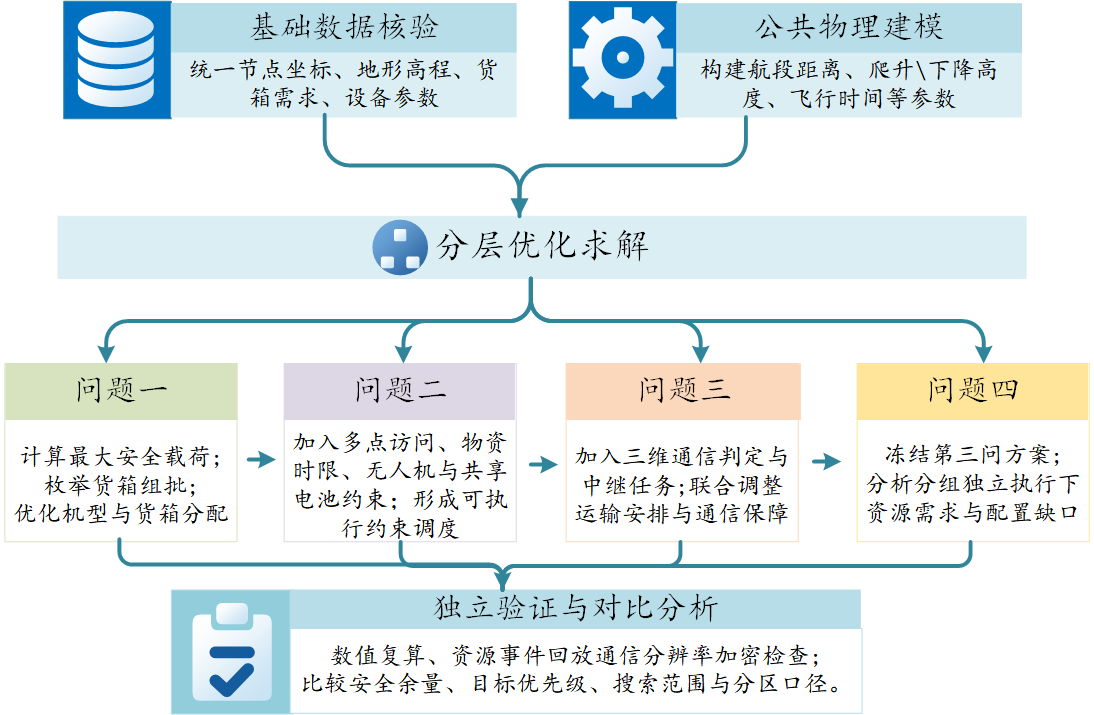
\includegraphics[width=0.8\textwidth]{2.5.png}
  \caption{全文建模与求解流程图}
  \label{fig:2-5}
\end{figure}


% 导言区需包含：
% \usepackage{amsmath,amssymb,booktabs,longtable,array}

\section{模型假设与符号说明}

\subsection{模型假设}

为统一四个问题的计算口径，在保留题目规定与附件数据的基础上，
对原文未明确的环节作如下假设。以下工作假设均需要用户核验，
其适用范围与可能影响在结果分析中说明。
货箱不可拆分、医疗与首批物资的硬时限、设备库存及返航电量下限等
属于题目给定约束，不作为另行提出的假设。

\begin{enumerate}

    \item \textbf{给定参数按确定值使用。}
    以附件提供的货箱需求、设备性能和通信参数作为基准输入，
    各航段按照给定速度及既定飞行剖面计算。
    不额外引入缺乏数据支持的随机故障、天气扰动和需求变化，
    因而所得结果对应确定性场景，不代表随机环境下的可靠性保证。

    \item \textbf{水平能耗按标准航程比例折算。}
    假设标准航程对应消耗整组可用电池能量。
    当机型为 $g$、航段载荷为 $q$ 时，水平飞行能耗为
    \begin{equation}
        E^{\mathrm{hor}}_{gij}(q)
        =
        E_g^{\mathrm{use}}
        \frac{d_{ij}}{L_g(q)},
    \end{equation}
    其中，载荷与航程的关系采用题目给定公式
    \begin{equation}
        L_g(q)
        =
        L_g^{0}
        -
        \left(L_g^{0}-L_g^{F}\right)
        \left(\frac{q}{Q_g}\right)^{3/2}.
    \end{equation}
    标准航程的能量标定属于工作假设；
    若标准航程本身已包含安全储备，则需调整上述折算关系。

    \item \textbf{爬升效率按能量转化效率解释。}
    将附件中的爬升效率解释为电能转化为重力势能的效率，
    爬升附加能耗表示为
    \begin{equation}
        E^{\mathrm{climb}}_{gij}(q)
        =
        \frac{(m_g+q)g_0h_{ij}^{+}}
        {\eta_g\,3.6\times10^{6}},
    \end{equation}
    其中 $g_0=9.80665\,\mathrm{m/s^2}$，
    分母中的换算系数用于将焦耳转换为千瓦时。
    空载质量使用附件给定口径，不重复加入已包含的电池质量；
    中继爬升计算使用其计划起飞总质量。

    \item \textbf{运输交接阶段不另计悬停能耗。}
    按题目能耗分解计算水平飞行与爬升附加能耗，
    下降不另计附加能耗。
    由于缺少运输机交接悬停功率参数，
    基准模型不额外加入该阶段的悬停能耗。
    这一简化可能低估实际任务耗电，
    获得相关功率数据后应重新计算返航安全余量。

    \item \textbf{交付完成时刻按整次交接结束计算。}
    将架次开始定义为固定准备开始，
    完成准备和逐箱装载后起飞。
    每次服务区交接时长由基础交接时间与逐箱附加时间组成，
    该次访问的全部货箱统一记为交接结束时完成交付，
    不以到达时刻代替交付完成时刻。

    \item \textbf{机体与能源资源分别调度。}
    运输机体从准备开始占用至返航落地，
    不额外加入附件未给定的运输周转时间。
    电池从准备开始预留，返航后可立即拆下充电，
    不另计拆装时间，再次分配前必须充满。
    中继机体返航后完成规定周转方可再次使用，
    能源组件充电可与机体周转并行。
    不额外设置附件未给定的充电器或准备工位数量限制。

    \item \textbf{节点作业高度与地形高程分别保留。}
    节点起降和作业高度采用节点表数据，
    航段地形与通信遮挡使用DEM数据，
    不通过改写节点海拔消除二者差异。
    按PixelIsPoint登记方式处理像元坐标，
    在通信判定中将像元内部地形表示为常高表面，
    射线经过像元边界或角点时采用保守检查。

    \item \textbf{通信容量与切换采用简化口径。}
    附件未给出中继并发服务数量、带宽及切换耗时限制时，
    假设一架中继可同时保障多架满足链路条件的运输机，
    保障源切换不另计额外时间。
    每架运输机同一时刻只采用直连或一架中继保障，
    不引入中继之间的多跳转发。
    该口径仅用于链路与任务安排，不构成真实网络容量认证。

    \item \textbf{中继建链功耗与转场剖面采用统一解释。}
    建链阶段和有效服务阶段均按悬停功率与通信附加功率之和计耗。
    中继转场采用垂直爬升、水平巡航和垂直下降的分段剖面，
    转场海拔取
    \begin{equation}
        H^{\mathrm{tr}}
        =
        \max\left\{
        H^{\mathrm{DEM}}_{\max}+50,\,
        H^{\mathrm{start}},\,
        H^{\mathrm{end}}
        \right\}.
    \end{equation}
    该解释保证转场高度不低于路径净空要求和两端高度，
    避免出现负爬升或负下降。

    \item \textbf{第四问允许组内资源重新编号。}
    冻结第三问基准方案的货箱组批、机型、访问顺序、
    任务位置、全部时刻及通信保障关系。
    在此基础上，允许组内同型号机体和能源资源重新编号并合法复用，
    但不改变任何任务的物理内容，各类实体资源不得跨组调配。
    同时以继承原实体编号的口径作为对照。

    \item \textbf{跨组中继采用完整任务副本。}
    第四问基准假设：当一个原中继架次实际保障多个任务组时，
    各相关组分别配置该架次的完整副本。
    副本保留原准备、转场、建链、服务、返航和周转时段，
    并完整计入资源与能耗；同组内重复引用只计一次。
    该假设与禁止复制中继的口径分别比较，
    不将其表述为题目明确规定。
    复制后的实际干扰、网络容量和空域运行条件仍需进一步核验。

\end{enumerate}

需要说明的是，候选位置离散化、每架次最大访问点数及搜索次数
属于求解过程中的计算限制，而非物理假设或题目原始约束，
将在相应问题的算法部分单独说明。
第三问的通信检查结论限定于实际采用的时空分辨率，
第四问继承该限制，不据此宣称连续通信已获数学证明。

\subsection{符号说明}

为避免不同章节之间出现符号歧义，主要符号统一如下。
局部算法状态及辅助变量在对应模型中另行定义。

\renewcommand{\arraystretch}{1.18}
\begin{longtable}{
    >{\raggedright\arraybackslash}p{2.8cm}
    >{\raggedright\arraybackslash}p{8.4cm}
    >{\raggedright\arraybackslash}p{2cm}
}
    \caption{主要符号及其含义}
    \label{tab:notation}\\
    \toprule
    符号 & 含义 & 单位或取值 \\
    \midrule
    \endfirsthead

    \multicolumn{3}{c}{表~\thetable\quad 续表}\\
    \toprule
    符号 & 含义 & 单位或取值 \\
    \midrule
    \endhead

    \bottomrule
    \endfoot

    $\mathcal{S}$ & 服务区集合，不包含调度中心 & 集合 \\
    $0$ & 调度中心O01的节点索引 & --- \\
    $i,j$ & 调度中心或服务区的节点索引 & --- \\
    $g$ & 运输无人机机型索引 & $A,B,C$ \\
    $b$ & 货箱索引 & --- \\
    $k,r$ & 运输架次、中继架次索引 & --- \\

    $w_b,v_b$ & 货箱$b$的质量与体积 & kg，m$^3$ \\
    $d_b$ & 货箱$b$的期望送达时刻 & s \\
    $\tau_b^{\mathrm{hard}}$ &
    货箱$b$适用的最早硬截止时刻；
    无硬时限时取$+\infty$ & s \\
    $\alpha_b$ & 货箱$b$的应急优先系数 & 无量纲 \\
    $T_b$ & 货箱$b$的交付完成时刻 & s \\

    $Q_g,V_g$ & 机型$g$的额定载质量与装载体积上限 & kg，m$^3$ \\
    $m_g$ & 机型$g$按附件口径给出的空载质量 & kg \\
    $E_g^{\mathrm{use}}$ & 机型$g$电池的可用能量 & kWh \\
    $L_g^0,L_g^F$ & 机型$g$的空载、满载标准航程 & m \\
    $L_g(q)$ & 机型$g$在载荷$q$下的标准航程 & m \\
    $\eta_g$ & 机型$g$的爬升效率 & 无量纲 \\
    $\rho_g$ & 机型$g$的返航SOC下限 & 比例 \\
    $q$ & 当前航段携带的货物质量 & kg \\
    $q_{ig}^{*}$ & 机型$g$对服务区$i$的最大安全往返载荷 & kg \\

    $d_{ij}$ & 节点$i$至$j$的水平航段距离 & m \\
    $h_{ij}^{+},h_{ij}^{-}$ & 有向航段$i\to j$的爬升、下降高度 & m \\
    $v_g^{\mathrm{cr}}$ & 机型$g$的巡航速度 & m/s \\
    $v_g^{+},v_g^{-}$ & 机型$g$的爬升、下降速度 & m/s \\
    $E_{gij}(q)$ & 机型$g$以载荷$q$执行航段$i\to j$的能耗 & kWh \\
    $g_0$ & 重力加速度 & m/s$^2$ \\

    $x_{bk}$ & 货箱$b$是否分配给运输架次$k$ & $\{0,1\}$ \\
    $\pi_k$ & 运输架次$k$的有序服务区访问序列 & 序列 \\
    $s_k,t_k^{\mathrm{off}},f_k$ &
    运输架次$k$的准备开始、起飞及返航时刻 & s \\
    $q_{kij}$ & 运输架次$k$在航段$i\to j$上的剩余载荷 & kg \\
    $\operatorname{SOC}_e(t)$ &
    电池或能源组件$e$在时刻$t$的荷电状态 & $[0,1]$ \\
    $T_e^{\mathrm{full}}$ &
    能源资源$e$的等效完全充电时间 & s \\
    $\tau_e^{\mathrm{chg}}$ &
    能源资源$e$返航后恢复满电所需时间 & s \\

    $\boldsymbol{p}_k(t)$ & 运输架次$k$在时刻$t$的三维位置 & m \\
    $\boldsymbol{p}_r^{\mathrm{hov}}$ &
    中继架次$r$的三维悬停位置 & m \\
    $c_r,e_r$ & 中继架次$r$的建链完成与服务结束时刻 & s \\
    $\mathcal{L}_{uv}(t)$ &
    通信端点$u,v$之间在时刻$t$的总链路损耗 & dB \\
    $\mathcal{L}_{uv}^{\max}$ &
    通信端点$u,v$双向链路允许的最大损耗 & dB \\
    $M_{uv}(t)$ &
    链路裕量，等于允许损耗减去实际总损耗 & dB \\
    $y_{kr}(t)$ &
    时刻$t$运输架次$k$是否由中继架次$r$保障 & $\{0,1\}$ \\

    $D$ & 全部货箱的加权延误 & 优先系数$\cdot$s \\
    $T_{\mathrm{sum}}$ & 第一问各架次累计作业时间之和 & s \\
    $C_{\max}$ & 第二问全部运输无人机的最晚返航时刻 & s \\
    $C_{\mathrm{joint}}$ &
    第三问全部运输与中继无人机的最晚返航时刻 & s \\
    $E^{\mathrm{T}},E^{\mathrm{R}}$ &
    运输任务总能耗与中继任务总能耗 & kWh \\
    $N^{\mathrm{T}},N^{\mathrm{R}}$ &
    运输架次数与中继架次数 & 架次 \\

    $K$ & 第四问任务组数量 & $2$或$3$ \\
    $\ell$ & 任务组索引 & $1,\ldots,K$ \\
    $a$ & 不可拆分服务区块索引 & --- \\
    $z_{a\ell}$ &
    服务区块$a$是否划入任务组$\ell$ & $\{0,1\}$ \\
    $c_{r\ell}$ &
    任务组$\ell$是否需要原中继架次$r$的完整副本 & $\{0,1\}$ \\
    $\gamma$ & 机体或能源资源类型索引 & 共8类 \\
    $n_{\ell\gamma}$ &
    任务组$\ell$对资源类型$\gamma$的配置需求 & 架或组 \\
    $R_\gamma,I_\gamma$ &
    资源类型$\gamma$的分区总需求与现有库存 & 架或组 \\
    $\Delta_\gamma,U_\gamma$ &
    资源类型$\gamma$的配置缺口与库存剩余 & 架或组 \\
    $W_\ell$ &
    任务组$\ell$的机体占用工作量，包含中继周转 & s \\
    $G,S$ & 归一化资源缺口与归一化配置规模 & 无量纲 \\
    $\mathrm{CV}$ & 各组工作量的变异系数 & 无量纲 \\

\end{longtable}

其中，加权延误仅对具有期望送达时间的货箱计算：
\begin{equation}
    D
    =
    \sum_{b:\,d_b\text{已给定}}
    \alpha_b\max\{0,T_b-d_b\}.
\end{equation}
医疗物资及首批保障物资的硬时限另由
$T_b\leq \tau_b^{\mathrm{hard}}$约束，
不能通过支付延误惩罚予以放宽。

第四问各类型资源的需求、缺口和剩余分别定义为
\begin{equation}
    R_\gamma
    =
    \sum_{\ell=1}^{K}n_{\ell\gamma},
    \qquad
    \Delta_\gamma
    =
    \max\{0,R_\gamma-I_\gamma\},
    \qquad
    U_\gamma
    =
    \max\{0,I_\gamma-R_\gamma\}.
\end{equation}
相应的归一化指标为
\begin{equation}
    G
    =
    \sum_{\gamma}\frac{\Delta_\gamma}{I_\gamma},
    \qquad
    S
    =
    \sum_{\gamma}\frac{R_\gamma}{I_\gamma}.
\end{equation}
上述指标用于比较不同类型资源的相对配置规模，
不表示货币成本，也不允许用一种资源的剩余抵消另一种资源的缺口。

工作量均衡指标定义为
\begin{equation}
    \overline{W}
    =
    \frac{1}{K}\sum_{\ell=1}^{K}W_\ell,
    \qquad
    \mathrm{CV}
    =
    \frac{
        \sqrt{\frac{1}{K}\sum_{\ell=1}^{K}
        (W_\ell-\overline{W})^2}
    }{\overline{W}}.
\end{equation}

需要特别区分：
$T_{\mathrm{sum}}$是各架次作业时间的累加，
$C_{\max}$和$C_{\mathrm{joint}}$是并行执行下的最晚返航时刻，
三者不能直接混用。
末次返航后的补电不计入任务完成时间，
但仍计入能源资源恢复可用时刻。



\section{数据核验与公共物理模型}

为保证四个问题的数据一致性与结果可复算性，首先对原始附件、
预处理数据及前序计算成果进行核验，并统一航段几何、飞行时间、
运输能耗和能源周转的计算规则。后续各问在此基础上加入相应的
组批、调度、通信或分区约束，不重复修改公共物理参数。

\subsection{数据来源与一致性核验}

基础数据包括调度中心与服务区信息、逐箱物资需求、运输无人机参数、
中继无人机参数、通信链路参数及数字高程模型。
其中，节点表提供位置与海拔，货箱表提供目的地、质量、体积和时限，
设备表提供性能及库存，DEM用于航段地形净空与通信遮挡分析。

核验后，研究对象包含1个调度中心、15个服务区和80个货箱。
其中，医疗物资为16箱，首批保障物资为30箱，两类标记可以重合，
不能将其数量直接相加作为具有硬时限的货箱总数。
运输及中继资源库存如表~\ref{tab:resource_inventory}所示。

\begin{table}[htbp]
    \centering
    \caption{无人机与能源资源库存}
    \label{tab:resource_inventory}
    \begin{tabular}{lcc}
        \toprule
        资源类别 & 实体无人机数量/架 & 电池或能源组件数量/组 \\
        \midrule
        A型运输无人机 & 4 & 6 \\
        B型运输无人机 & 2 & 4 \\
        C型运输无人机 & 2 & 4 \\
        中继无人机   & 2 & 6 \\
        \bottomrule
    \end{tabular}
\end{table}

共享电池总数已经包含初始机载使用和备用周转所需电池，
不能在附件库存之外再次增加初始电池。
同机型共享电池可以在不同实体无人机之间复用，
不同机型之间不能混用。

数据核验主要包括以下内容：
检查货箱编号的唯一性，核对逐箱质量、体积和需求汇总；
检查货箱目的地与服务区编号的对应关系；
核对设备性能、库存数量及时间单位；
检查预处理航段与原始节点数据的一致性。
对缺失的期望时间或截止时间保留缺失状态，不将其替换为0。

对于货箱$b$，将其适用的硬截止时间构成集合
$\mathcal{D}_b^{\mathrm{hard}}$。
医疗物资的期望送达时间和首批保障物资的首批截止时间
分别加入该集合，并定义
\begin{equation}
    \tau_b^{\mathrm{hard}}
    =
    \begin{cases}
        \displaystyle
        \min_{d\in\mathcal{D}_b^{\mathrm{hard}}} d,
        & \mathcal{D}_b^{\mathrm{hard}}\neq\varnothing,\\[6pt]
        +\infty,
        & \mathcal{D}_b^{\mathrm{hard}}=\varnothing.
    \end{cases}
\end{equation}
因此，同一货箱同时具有两类硬时限时，必须满足其中更早的截止时间。
普通物资的期望送达时间仅用于计算延误指标，不擅自转为硬约束。

同时，对纳入预处理核验的9个原始文件计算SHA-256，
并与已保存的核验记录比较，结果保持一致。
经核验的公共数据包含16个节点、240条有向航段，
以及三种运输机型对应的720条航段飞行时间记录。
因此，后续计算复用已有预处理结果，不重复修改原始附件。

% 导言区需加载：
% \usepackage{graphicx}
% \usepackage{amsmath}

\subsection{地形处理与有向航段构建}

研究区域的地形背景及调度中心、服务区的空间分布如
图\ref{fig:study-area-nodes}所示。
调度中心O01与15个服务区分布于起伏的山地环境中，
节点间的运输能力不仅取决于水平距离，
还受到沿途地形高程及起降高度的影响。
为统一后续运输与通信模型的空间计算口径，
本节依次进行局部坐标转换、DEM空间登记处理及有向航段飞行剖面构建。
图中乡界仅用于说明研究区域，不作为任务分区的约束。

\begin{figure}[htbp]
    \centering
    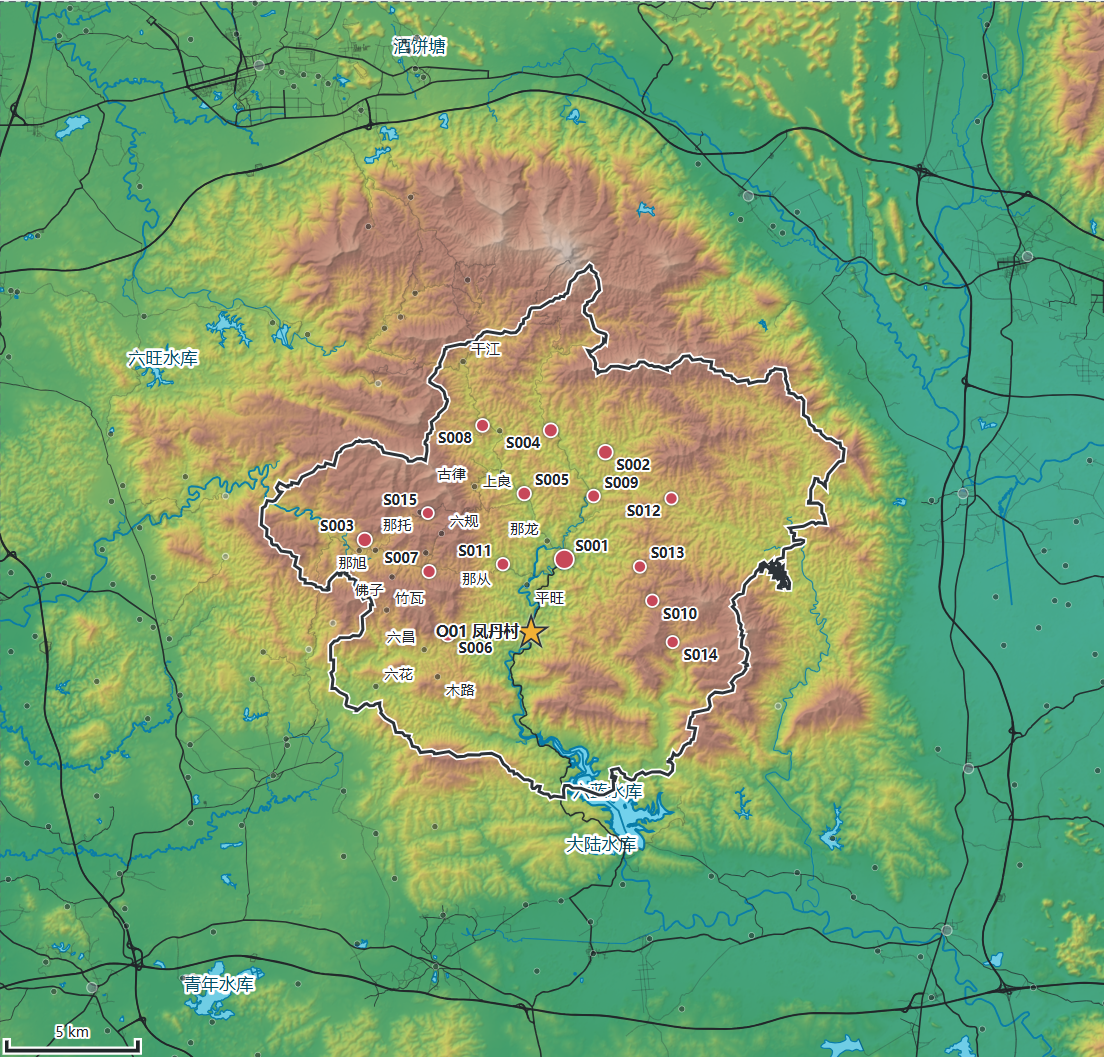
\includegraphics[width=0.82\textwidth]{4.2.png}
    \caption{研究区域与节点分布图}
    \label{fig:study-area-nodes}

    \vspace{2mm}
    \begin{minipage}{0.82\textwidth}
        \small
        注：星形为调度中心O01，红点为服务区，
        白色轮廓为镇龙乡边界；
        底图及节点数据来源于题目附件。
    \end{minipage}
\end{figure}

\subsubsection{局部坐标与水平距离}

为统一距离和能耗计算中的长度单位，
将节点经纬度转换为局部米制坐标。
设节点$i$的经纬度为$(\lambda_i,\varphi_i)$，则
\begin{equation}
    x_i=k_{\lambda}(\lambda_i-\lambda_0),
    \qquad
    y_i=k_{\varphi}(\varphi_i-\varphi_0),
\end{equation}
其中，$\lambda_0,\varphi_0$为局部坐标原点的经纬度，
$k_{\lambda},k_{\varphi}$为经纬度差到米制距离的换算系数。
计算中沿用已核验预处理记录中的原点与换算系数，
避免各问重新投影产生差异。

节点$i$至$j$的水平距离为
\begin{equation}
    d_{ij}
    =
    \sqrt{(x_j-x_i)^2+(y_j-y_i)^2}.
\end{equation}
该距离用于水平飞行时间和标准航程比例能耗计算。
通信自由空间损耗则使用通信端点之间的三维距离，
二者不混用。

\subsubsection{DEM登记与节点高度}

图\ref{fig:study-area-nodes}用于展示区域地形与节点位置，
具体航段高程和通信遮挡均由原始DEM数据计算，
不通过图面颜色估读。

原始GeoTIFF采用PixelIsPoint登记方式，
登记坐标对应像元中心。
因此，在建立像元边界与空间位置的对应关系时，
需考虑半个像元的偏移，避免将中心坐标误作边界坐标。

节点表海拔与DEM像元高程并不完全相同，
已核验节点的最大绝对差异约为$10.5629\,\mathrm{m}$。
模型保留这一差异：节点起降和作业高度采用节点表，
航段地形及通信遮挡采用DEM，
不通过修改节点海拔人为消除地形遮挡。

设节点$i$的表列地面海拔为$z_i$，
其作业海拔为
\begin{equation}
    z_i^{\mathrm{op}}
    =
    \begin{cases}
        z_i, & i=0,\\
        z_i+30, & i\in\mathcal{S}.
    \end{cases}
\end{equation}
其中，$i=0$表示调度中心O01，
$\mathcal{S}$表示服务区集合，
服务区的交接作业高度为地面以上$30\,\mathrm{m}$。

\subsubsection{巡航高度与爬升下降}

对运输航段$i\to j$，
沿水平航迹提取穿越地形的最高高程
$z_{ij}^{\mathrm{DEM,max}}$，
按题给净空要求确定巡航海拔
\begin{equation}
    H_{ij}
    =
    z_{ij}^{\mathrm{DEM,max}}+50.
\end{equation}
相应的爬升和下降高度为
\begin{equation}
    h_{ij}^{+}
    =
    H_{ij}-z_i^{\mathrm{op}},
    \qquad
    h_{ij}^{-}
    =
    H_{ij}-z_j^{\mathrm{op}}.
\end{equation}
上述高度均以米为单位。
使用该飞行剖面前，应核验爬升、下降高度的非负性；
若端点高度与巡航高度规则发生冲突，应核查剖面，
不能直接将负值截断后继续计算。

每次完成服务区交付后，
下一航段均从该服务区的作业高度重新爬升。
因此，多点运输不能将相邻服务区间的飞行
简化为始终保持巡航高度。

往返航段分别记录。
即使$d_{ij}=d_{ji}$，
其爬升、下降高度也需按照各自出发端与到达端计算。
当爬升和下降速度不同时，
正反向飞行时间一般不能直接视为相等。
\subsection{飞行时间与任务时间模型}

\subsubsection{航段飞行时间}

设机型$g$的巡航、爬升和下降速度分别为
$v_g^{\mathrm{cr}}$、$v_g^{+}$和$v_g^{-}$，
则航段$i\to j$的飞行时间为
\begin{equation}
    t_{gij}^{\mathrm{fly}}
    =
    \frac{h_{ij}^{+}}{v_g^{+}}
    +
    \frac{d_{ij}}{v_g^{\mathrm{cr}}}
    +
    \frac{h_{ij}^{-}}{v_g^{-}}.
\end{equation}
三项依次对应起点垂直爬升、水平巡航和终点垂直下降。

\subsubsection{准备、装载与交接时间}

设运输架次$k$采用机型$g_k$，
准备开始时刻为$s_k$，装载货箱数为$n_k$。
若固定准备时间为$t_{g_k}^{\mathrm{prep}}$，
每箱装载时间为$t_{g_k}^{\mathrm{load}}$，
则起飞时刻为
\begin{equation}
    t_k^{\mathrm{off}}
    =
    s_k+t_{g_k}^{\mathrm{prep}}
    +n_k t_{g_k}^{\mathrm{load}}.
\end{equation}

设架次$k$在服务区$i$交付$n_{ki}$个货箱，
基础交接时间为$t_{g_k}^{\mathrm{base}}$，
每箱附加交接时间为$t_{g_k}^{\mathrm{box}}$，
则该次访问的交接时长为
\begin{equation}
    t_{ki}^{\mathrm{service}}
    =
    t_{g_k}^{\mathrm{base}}
    +n_{ki}t_{g_k}^{\mathrm{box}}.
\end{equation}
若到达时刻为$a_{ki}$，则本次交付的每个货箱$b$均满足
\begin{equation}
    T_b
    =
    a_{ki}+t_{ki}^{\mathrm{service}}.
\end{equation}

沿访问顺序递推各航段飞行和服务时间，
可得到架次返航时刻$f_k$：
\begin{equation}
    f_k
    =
    t_k^{\mathrm{off}}
    +
    \sum_{(i,j)\in\mathcal{A}_k}
    t_{g_kij}^{\mathrm{fly}}
    +
    \sum_{i\in\pi_k}
    t_{ki}^{\mathrm{service}},
\end{equation}
其中，$\mathcal{A}_k$包含从O01出发、访问服务区及返回O01的全部航段。

\subsubsection{不同问题的时间指标}

第一问的累计作业时间为
\begin{equation}
    T_{\mathrm{sum}}
    =
    \sum_k(f_k-s_k),
\end{equation}
其含义是各架次准备、装载、飞行与交接时间之和，
不包含充电和排队，也不等于多机并行执行后的任务历时。

第二问以所有运输机的最晚返航时刻作为完成时间：
\begin{equation}
    C_{\max}
    =
    \max_k f_k.
\end{equation}

第三问同时考虑运输和中继任务：
\begin{equation}
    C_{\mathrm{joint}}
    =
    \max\left\{
    \max_k f_k,\,
    \max_r f_r
    \right\}.
\end{equation}
其中$f_r$为中继架次$r$的返航时刻。
末次返航后的补电及中继机体周转不计入联合完成时间，
但仍需在资源状态中记录。

\subsection{载荷更新、运输能耗与返航安全}

\subsubsection{逐航段载荷更新}

设$\mathcal{B}_k$为分配给架次$k$的货箱集合，
$\mathcal{D}_{ki}$为其从节点$i$出发前已经交付的货箱集合，
则当前航段的剩余载荷为
\begin{equation}
    q_{kij}
    =
    \sum_{b\in\mathcal{B}_k\setminus\mathcal{D}_{ki}}w_b.
\end{equation}
剩余货物体积同理为
\begin{equation}
    V_{kij}^{\mathrm{load}}
    =
    \sum_{b\in\mathcal{B}_k\setminus\mathcal{D}_{ki}}v_b.
\end{equation}
各航段应满足
\begin{equation}
    0\leq q_{kij}\leq Q_{g_k},
    \qquad
    0\leq V_{kij}^{\mathrm{load}}\leq V_{g_k}.
\end{equation}
全部货物交付后，返回O01的航段载荷为0。

\subsubsection{载荷相关能耗}

采用题给载荷与航程关系
\begin{equation}
    L_g(q)
    =
    L_g^0-
    (L_g^0-L_g^F)
    \left(\frac{q}{Q_g}\right)^{3/2}.
\end{equation}
在前述标准航程能量标定和爬升效率工作假设下，
运输机执行航段$i\to j$的能耗为
\begin{equation}
    E_{gij}(q)
    =
    E_g^{\mathrm{use}}
    \frac{d_{ij}}{L_g(q)}
    +
    \frac{(m_g+q)g_0h_{ij}^{+}}
    {\eta_g\,3.6\times10^{6}}.
\end{equation}
第一项为水平飞行能耗，第二项为爬升附加能耗。
距离统一使用米，质量使用千克，能量结果为千瓦时。

架次$k$的运输能耗按实际剩余载荷逐段累计：
\begin{equation}
    E_k
    =
    \sum_{(i,j)\in\mathcal{A}_k}
    E_{g_kij}(q_{kij}).
\end{equation}
因此，不能用起飞载荷计算全部航段，
也不能用单程能耗乘以2代替载货去程与空载返程。

中继无人机的水平飞行采用功率与时间相乘计算，
不套用运输机的载荷—航程标定式。
其中继爬升、建链及悬停通信能耗在第三问中分别建立。

\subsubsection{返航SOC与安全余量}

能源初始为满电时，运输架次$k$的返航SOC为
\begin{equation}
    \operatorname{SOC}_k^{\mathrm{return}}
    =
    1-\frac{E_k}{E_{g_k}^{\mathrm{use}}}.
\end{equation}
返航安全约束表示为
\begin{equation}
    \operatorname{SOC}_k^{\mathrm{return}}
    \geq \rho_{g_k},
\end{equation}
等价地，
\begin{equation}
    E_k
    \leq
    (1-\rho_{g_k})E_{g_k}^{\mathrm{use}}.
\end{equation}
基准安全余量按附件取值，敏感性分析中的其他余量仅作为对比情景。
对于空载往返已不满足能量约束的情况，应标记为不可行，
不能用最大安全载荷为0掩盖不可达性。

\subsection{两阶段充电与资源占用}

\subsubsection{两阶段充电模型}

设能源资源$e$的返航SOC为$s$，
等效完全充电时间为$T_e^{\mathrm{full}}$。
根据题给两阶段规则，恢复至满电所需时间为
\begin{equation}
    \tau_e^{\mathrm{chg}}(s)
    =
    \begin{cases}
        T_e^{\mathrm{full}}
        \left[
        0.65\displaystyle\frac{0.9-s}{0.9}+0.35
        \right],
        & 0\leq s<0.9,\\[8pt]
        T_e^{\mathrm{full}}
        \cdot0.35\displaystyle\frac{1-s}{0.1},
        & 0.9\leq s\leq1.
    \end{cases}
\end{equation}
该式适用于运输电池和中继能源组件，
但其完全充电时间分别读取相应机型参数。

沿用返航后立即开始充电的工作假设，
若任务返航时刻为$f$，则能源恢复可用时刻为
\begin{equation}
    t_e^{\mathrm{ready}}
    =
    f+\tau_e^{\mathrm{chg}}(s).
\end{equation}
下一次使用该能源的准备开始时刻不得早于
$t_e^{\mathrm{ready}}$。

\subsubsection{机体与能源的独立占用}

运输机体和电池的可用时刻通常不同，
因此将其作为独立资源记录。各类资源的占用区间统一定义为
\begin{align}
    \mathcal{I}_k^{\mathrm{T,body}}
    &=[s_k,f_k),\\
    \mathcal{I}_k^{\mathrm{T,battery}}
    &=[s_k,t_{e(k)}^{\mathrm{ready}}),\\
    \mathcal{I}_r^{\mathrm{R,body}}
    &=[s_r,f_r+t^{\mathrm{turn}}),\\
    \mathcal{I}_r^{\mathrm{R,energy}}
    &=[s_r,t_{e(r)}^{\mathrm{ready}}),
\end{align}
其中，$e(k)$和$e(r)$分别表示任务使用的电池或能源组件，
$t^{\mathrm{turn}}$为中继机体规定的周转时间。

同一实体资源的占用区间不得重叠。
区间采用左闭右开的形式，
在严格同一时刻完成释放并开始下一任务时，先释放后占用。
计算使用未四舍五入的数据，展示精度不参与可行性判断。
独立复算的时间、能量和SOC容差分别取
$10^{-7}\,\mathrm{s}$、
$10^{-8}\,\mathrm{kWh}$和$10^{-10}$。

第一问仅使用上述公共时间与能耗规则，
不引入实体设备库存和充电调度约束；
第二、三问将库存作为硬约束；
第四问则冻结第三问任务时序，按组独立核算资源需求，
并将超过现有库存的部分明确列为配置缺口。
这一处理保证各问共享物理基础，同时保留各自不同的研究范围。

% 导言区需包含：
% \usepackage{amsmath,amssymb,booktabs}

\section{问题一：单点往返运输能力与货箱组批}

本问研究运输无人机执行
$\mathrm{O01}\rightarrow S_i\rightarrow\mathrm{O01}$
单点往返任务时的运输能力与货箱分配。
每架次仅向一个服务区配送，去程携带本架次全部货物，
交付后空载返回调度中心。
首先计算各机型面向不同服务区的最大安全载荷，
再结合货箱体积及不可拆分要求确定组批和机型选择。

本问不引入实体无人机数量、共享电池调度、充电、
通信及后续问题的配送时限约束。
能耗计算沿用公共物理模型中的工作假设，
所得结论限定于该能量标定与计算口径。

\subsection{单点往返最大安全载荷模型}

\subsubsection{往返运输能耗}

设机型$g$携带质量为$q$的货物，从O01前往服务区$i$。
根据题给载荷—航程关系，
\begin{equation}
    L_g(q)
    =
    L_g^0-
    \left(L_g^0-L_g^F\right)
    \left(\frac{q}{Q_g}\right)^{3/2},
    \qquad 0\leq q\leq Q_g.
    \label{eq:q1_range}
\end{equation}

去程载荷为$q$，返程载荷为0，
两个方向分别采用对应航段的距离和爬升高度。
在标准航程能量标定及爬升效率解释的工作假设下，
全架次往返能耗为
\begin{equation}
\begin{aligned}
    E_{gi}^{\mathrm{rt}}(q)
    ={}&
    E_g^{\mathrm{use}}\frac{d_{0i}}{L_g(q)}
    +
    \frac{(m_g+q)g_0h_{0i}^{+}}
    {\eta_g\,3.6\times10^6}
    \\
    &+
    E_g^{\mathrm{use}}\frac{d_{i0}}{L_g^0}
    +
    \frac{m_g g_0h_{i0}^{+}}
    {\eta_g\,3.6\times10^6}.
\end{aligned}
\label{eq:q1_roundtrip_energy}
\end{equation}

式~\eqref{eq:q1_roundtrip_energy}中的四项依次为
去程水平飞行能耗、去程爬升附加能耗、
空载返程水平飞行能耗和空载返程爬升附加能耗。
其中$m_g$已经按附件口径包含电池质量，
不再重复加入电池质量。

返程虽然不携带货物，但仍需从服务区作业高度爬升至巡航高度，
因此不能忽略返程爬升能耗。
下降不另计附加能耗，运输交接阶段未额外加入缺少功率参数的悬停能耗。

\subsubsection{安全载荷约束}

设机型$g$的返航SOC下限为$\rho_g$，
则全架次允许消耗的能量上限为
\begin{equation}
    B_g=(1-\rho_g)E_g^{\mathrm{use}}.
\end{equation}
最大安全载荷定义为
\begin{equation}
\begin{aligned}
    q_{ig}^{*}
    ={}&\max_q \quad q,\\
    \text{s.t.}\quad
    &0\leq q\leq Q_g,\\
    &E_{gi}^{\mathrm{rt}}(q)\leq B_g.
\end{aligned}
\label{eq:q1_safe_payload}
\end{equation}

式~\eqref{eq:q1_safe_payload}同时考虑额定载质量和全架次返航安全余量。
它描述的是连续质量意义上的运输能力，
尚未包含具体货箱的体积和不可拆分限制。
实际可装货物还需在组批模型中进一步检验。

求解前先判断空载往返是否可行。
若$E_{gi}^{\mathrm{rt}}(0)>B_g$，
则该机型无法在规定安全余量下完成该服务区的往返任务，
应标记为不可行，不能将其解释为最大载荷为0。

\subsubsection{基于单调性的求解方法}

由附件参数可知$L_g^0>L_g^F>0$，且
\begin{equation}
    \frac{\mathrm{d}L_g(q)}{\mathrm{d}q}
    =
    -\frac{3(L_g^0-L_g^F)}{2Q_g}
    \left(\frac{q}{Q_g}\right)^{1/2}
    \leq 0.
\end{equation}
因此，水平能耗随载荷增加而增大，
爬升附加能耗也随载荷线性增加。
在本数据对应的非负爬升条件下，
$E_{gi}^{\mathrm{rt}}(q)$关于$q$单调不减。

据此，将最大安全载荷计算分为三种情况：
\begin{equation}
    q_{ig}^{*}
    =
    \begin{cases}
        \text{不可行},
        &E_{gi}^{\mathrm{rt}}(0)>B_g,\\[3pt]
        Q_g,
        &E_{gi}^{\mathrm{rt}}(Q_g)\leq B_g,\\[3pt]
        \displaystyle
        \sup\left\{q\in[0,Q_g]:
        E_{gi}^{\mathrm{rt}}(q)\leq B_g\right\},
        &\text{其他情况}.
    \end{cases}
\end{equation}

第三种情况下，使用二分法搜索能量约束对应的载荷边界。
每次保留满足约束的一侧，最终输出可行侧的载荷值。
程序采用80轮二分，实际精度受浮点运算精度限制，
可行性判断使用未四舍五入数据。

\subsection{货箱组批与机型选择模型}

\subsubsection{可行运输模式构建}

设$\mathcal{B}_i$为目的地为服务区$i$的货箱集合。
一个运输模式$k$由服务区$i$、机型$g(k)$
以及非空货箱子集$\mathcal{B}_k\subseteq\mathcal{B}_i$组成。

该模式的箱数、总质量和总体积分别为
\begin{equation}
    n_k=|\mathcal{B}_k|,
    \qquad
    q_k=\sum_{b\in\mathcal{B}_k}w_b,
    \qquad
    v_k=\sum_{b\in\mathcal{B}_k}v_b.
\end{equation}

仅保留满足以下约束的模式：
\begin{align}
    q_k &\leq Q_{g(k)},\\
    v_k &\leq V_{g(k)},\\
    E_{g(k)i}^{\mathrm{rt}}(q_k)
    &\leq
    (1-\rho_{g(k)})E_{g(k)}^{\mathrm{use}}.
\end{align}
记服务区$i$的全部可行模式集合为$\mathcal{P}_i$。

由于模式按服务区分别生成，
其内部已经满足不得跨服务区组批的要求；
模式中的每个货箱均以完整个体加入，不允许拆分。

\subsubsection{模式时间与能耗}

可行模式$k$的能耗为
\begin{equation}
    e_k=E_{g(k)i}^{\mathrm{rt}}(q_k).
\end{equation}
其完整作业时间为
\begin{equation}
\begin{aligned}
    \tau_k={}&
    t_{g(k)}^{\mathrm{prep}}
    +n_k t_{g(k)}^{\mathrm{load}}
    +t_{g(k),0i}^{\mathrm{fly}}
    +t_{g(k),i0}^{\mathrm{fly}}\\
    &+
    t_{g(k)}^{\mathrm{base}}
    +n_k t_{g(k)}^{\mathrm{box}}.
\end{aligned}
\label{eq:q1_pattern_time}
\end{equation}

式~\eqref{eq:q1_pattern_time}包含固定准备、逐箱装载、
往返飞行以及服务区交接时间，不包含充电和排队。
其中，往返纯飞行时间仅为
$t_{g(k),0i}^{\mathrm{fly}}+t_{g(k),i0}^{\mathrm{fly}}$，
不能与完整作业时间混用。

\subsubsection{分配约束与字典序目标}

在逐箱模式表示下，定义二元决策变量
\begin{equation}
    y_k=
    \begin{cases}
        1,&\text{选用模式}k,\\
        0,&\text{不选用模式}k.
    \end{cases}
\end{equation}
令$a_{bk}=1$表示模式$k$包含货箱$b$，否则$a_{bk}=0$。
为保证每个货箱恰好配送一次，建立约束
\begin{equation}
    \sum_{k\in\mathcal{P}_i}a_{bk}y_k=1,
    \qquad
    \forall b\in\mathcal{B}_i,\quad
    \forall i\in\mathcal{S}.
\label{eq:q1_exact_assignment}
\end{equation}

总架次数、总能耗及累计作业时间分别为
\begin{align}
    N&=\sum_{i\in\mathcal{S}}
       \sum_{k\in\mathcal{P}_i}y_k,\\
    E&=\sum_{i\in\mathcal{S}}
       \sum_{k\in\mathcal{P}_i}e_k y_k,\\
    T_{\mathrm{sum}}
      &=\sum_{i\in\mathcal{S}}
       \sum_{k\in\mathcal{P}_i}\tau_k y_k.
\end{align}

基准采用字典序目标
\begin{equation}
    \operatorname{lex\,min}
    \left(N,E,T_{\mathrm{sum}}\right).
\label{eq:q1_lex_objective}
\end{equation}
即首先最小化总架次数，
在架次数最少的方案中最小化能耗，
再在前两项最优的方案中最小化累计作业时间。
该优先级属于建模选择，不是题目指定的唯一排序。

\subsection{完整模式枚举与动态规划求解}

\subsubsection{等价货箱压缩}

本问不引入物资类别对应的配送时限，
同一服务区内质量和体积均相同的货箱，
对容量、能耗和作业时间具有相同影响。
因此，将这些货箱合并为等价类，
以各类剩余箱数代替逐箱二元状态。

设服务区$i$共有$J_i$类等价货箱，
剩余需求状态为
\begin{equation}
    \boldsymbol{r}
    =
    (r_1,r_2,\ldots,r_{J_i}).
\end{equation}
模式$k$用箱数向量
\begin{equation}
    \boldsymbol{a}_k
    =
    (a_{1k},a_{2k},\ldots,a_{J_i k})
\end{equation}
表示，各分量为该模式装载的对应类别箱数。
模式求解完成后，再将等价类中的原始货箱编号逐一分配回架次。

该压缩仅用于第一问，在当前约束和目标下不丢失信息；
后续引入逐箱时限后，不能未经检验直接沿用相同等价关系。

\subsubsection{动态规划递推}

定义$F_i(\boldsymbol{r})$为完成剩余需求
$\boldsymbol{r}$所需的最优成本三元组。
边界条件为
\begin{equation}
    F_i(\boldsymbol{0})=(0,0,0).
\end{equation}

对非空状态，取第一个剩余箱数为正的类别
\begin{equation}
    j^{*}
    =
    \min\{j:r_j>0\}.
\end{equation}
在所有包含该类别、且不超过剩余需求的可行模式中递推：
\begin{equation}
    F_i(\boldsymbol{r})
    =
    \operatorname{lex\,min}_{\substack{
        k\in\mathcal{P}_i\\
        \boldsymbol{a}_k\leq\boldsymbol{r}\\
        a_{j^{*}k}\geq1
    }}
    \left[
        (1,e_k,\tau_k)
        +
        F_i(\boldsymbol{r}-\boldsymbol{a}_k)
    \right].
\label{eq:q1_dp}
\end{equation}
其中，向量加法按分量进行，
$\boldsymbol{a}_k\leq\boldsymbol{r}$也按分量比较。
若不存在满足条件的转移，则该状态不可行。

任一完整分组方案中，必然存在至少一个模式包含类别$j^{*}$，
因此上述锚定方式不会遗漏合法方案，
仅减少同一组批方案因架次排列不同产生的重复搜索。

各服务区之间不存在设备数量、充电或时间资源耦合，
三个目标又均为可加指标，
因此可分别求解各服务区，再汇总得到总体方案。
模式枚举与状态转移均完整执行，
未采用超时截断或启发式剪枝。

\subsection{计算结果与分析}

\subsubsection{最大安全载荷结果}

以附件规定的$20\%$返航安全余量为基准，
计算三种机型对15个服务区的单点往返最大安全载荷，
共得到45项结果，如表~\ref{tab:q1_safe_payload}所示。
各组合均满足空载往返条件，
表中载荷为额定载质量与往返能量约束共同作用下的连续质量上限，
具体货箱组批还需满足体积与不可拆分约束。

\begin{table}[H]
    \centering
    \caption{各机型单点往返最大安全载荷}
    \label{tab:q1_safe_payload}
    \begin{tabular}{lrrr}
        \toprule
        服务区 & A型/kg & B型/kg & C型/kg \\
        \midrule
        S001 & 25.000000 & 30.000000 & 80.000000 \\
        S002 & 25.000000 & 30.000000 & 68.861224 \\
        S003 & 25.000000 & 30.000000 & 68.217586 \\
        S004 & 25.000000 & 30.000000 & 63.698047 \\
        S005 & 25.000000 & 30.000000 & 80.000000 \\
        S006 & 25.000000 & 30.000000 & 80.000000 \\
        S007 & 25.000000 & 30.000000 & 80.000000 \\
        S008 & 25.000000 & 28.801769 & 58.905298 \\
        S009 & 25.000000 & 30.000000 & 80.000000 \\
        S010 & 25.000000 & 30.000000 & 80.000000 \\
        S011 & 25.000000 & 30.000000 & 80.000000 \\
        S012 & 25.000000 & 30.000000 & 68.122153 \\
        S013 & 25.000000 & 30.000000 & 80.000000 \\
        S014 & 25.000000 & 30.000000 & 80.000000 \\
        S015 & 25.000000 & 30.000000 & 80.000000 \\
        \bottomrule
    \end{tabular}
\end{table}

为消除不同机型额定载质量差异对直观比较的影响，
将最大安全载荷与对应额定载质量之比绘制为
图~\ref{fig:q1_safe_payload_ratio}。
该比例反映各机型在指定航线上的安全载荷能力，
不代表实际组批方案的装载率。
表中数值及图中标注均为展示值，
实际可行性判断采用未舍入结果。

\begin{figure}[H]
    \centering
    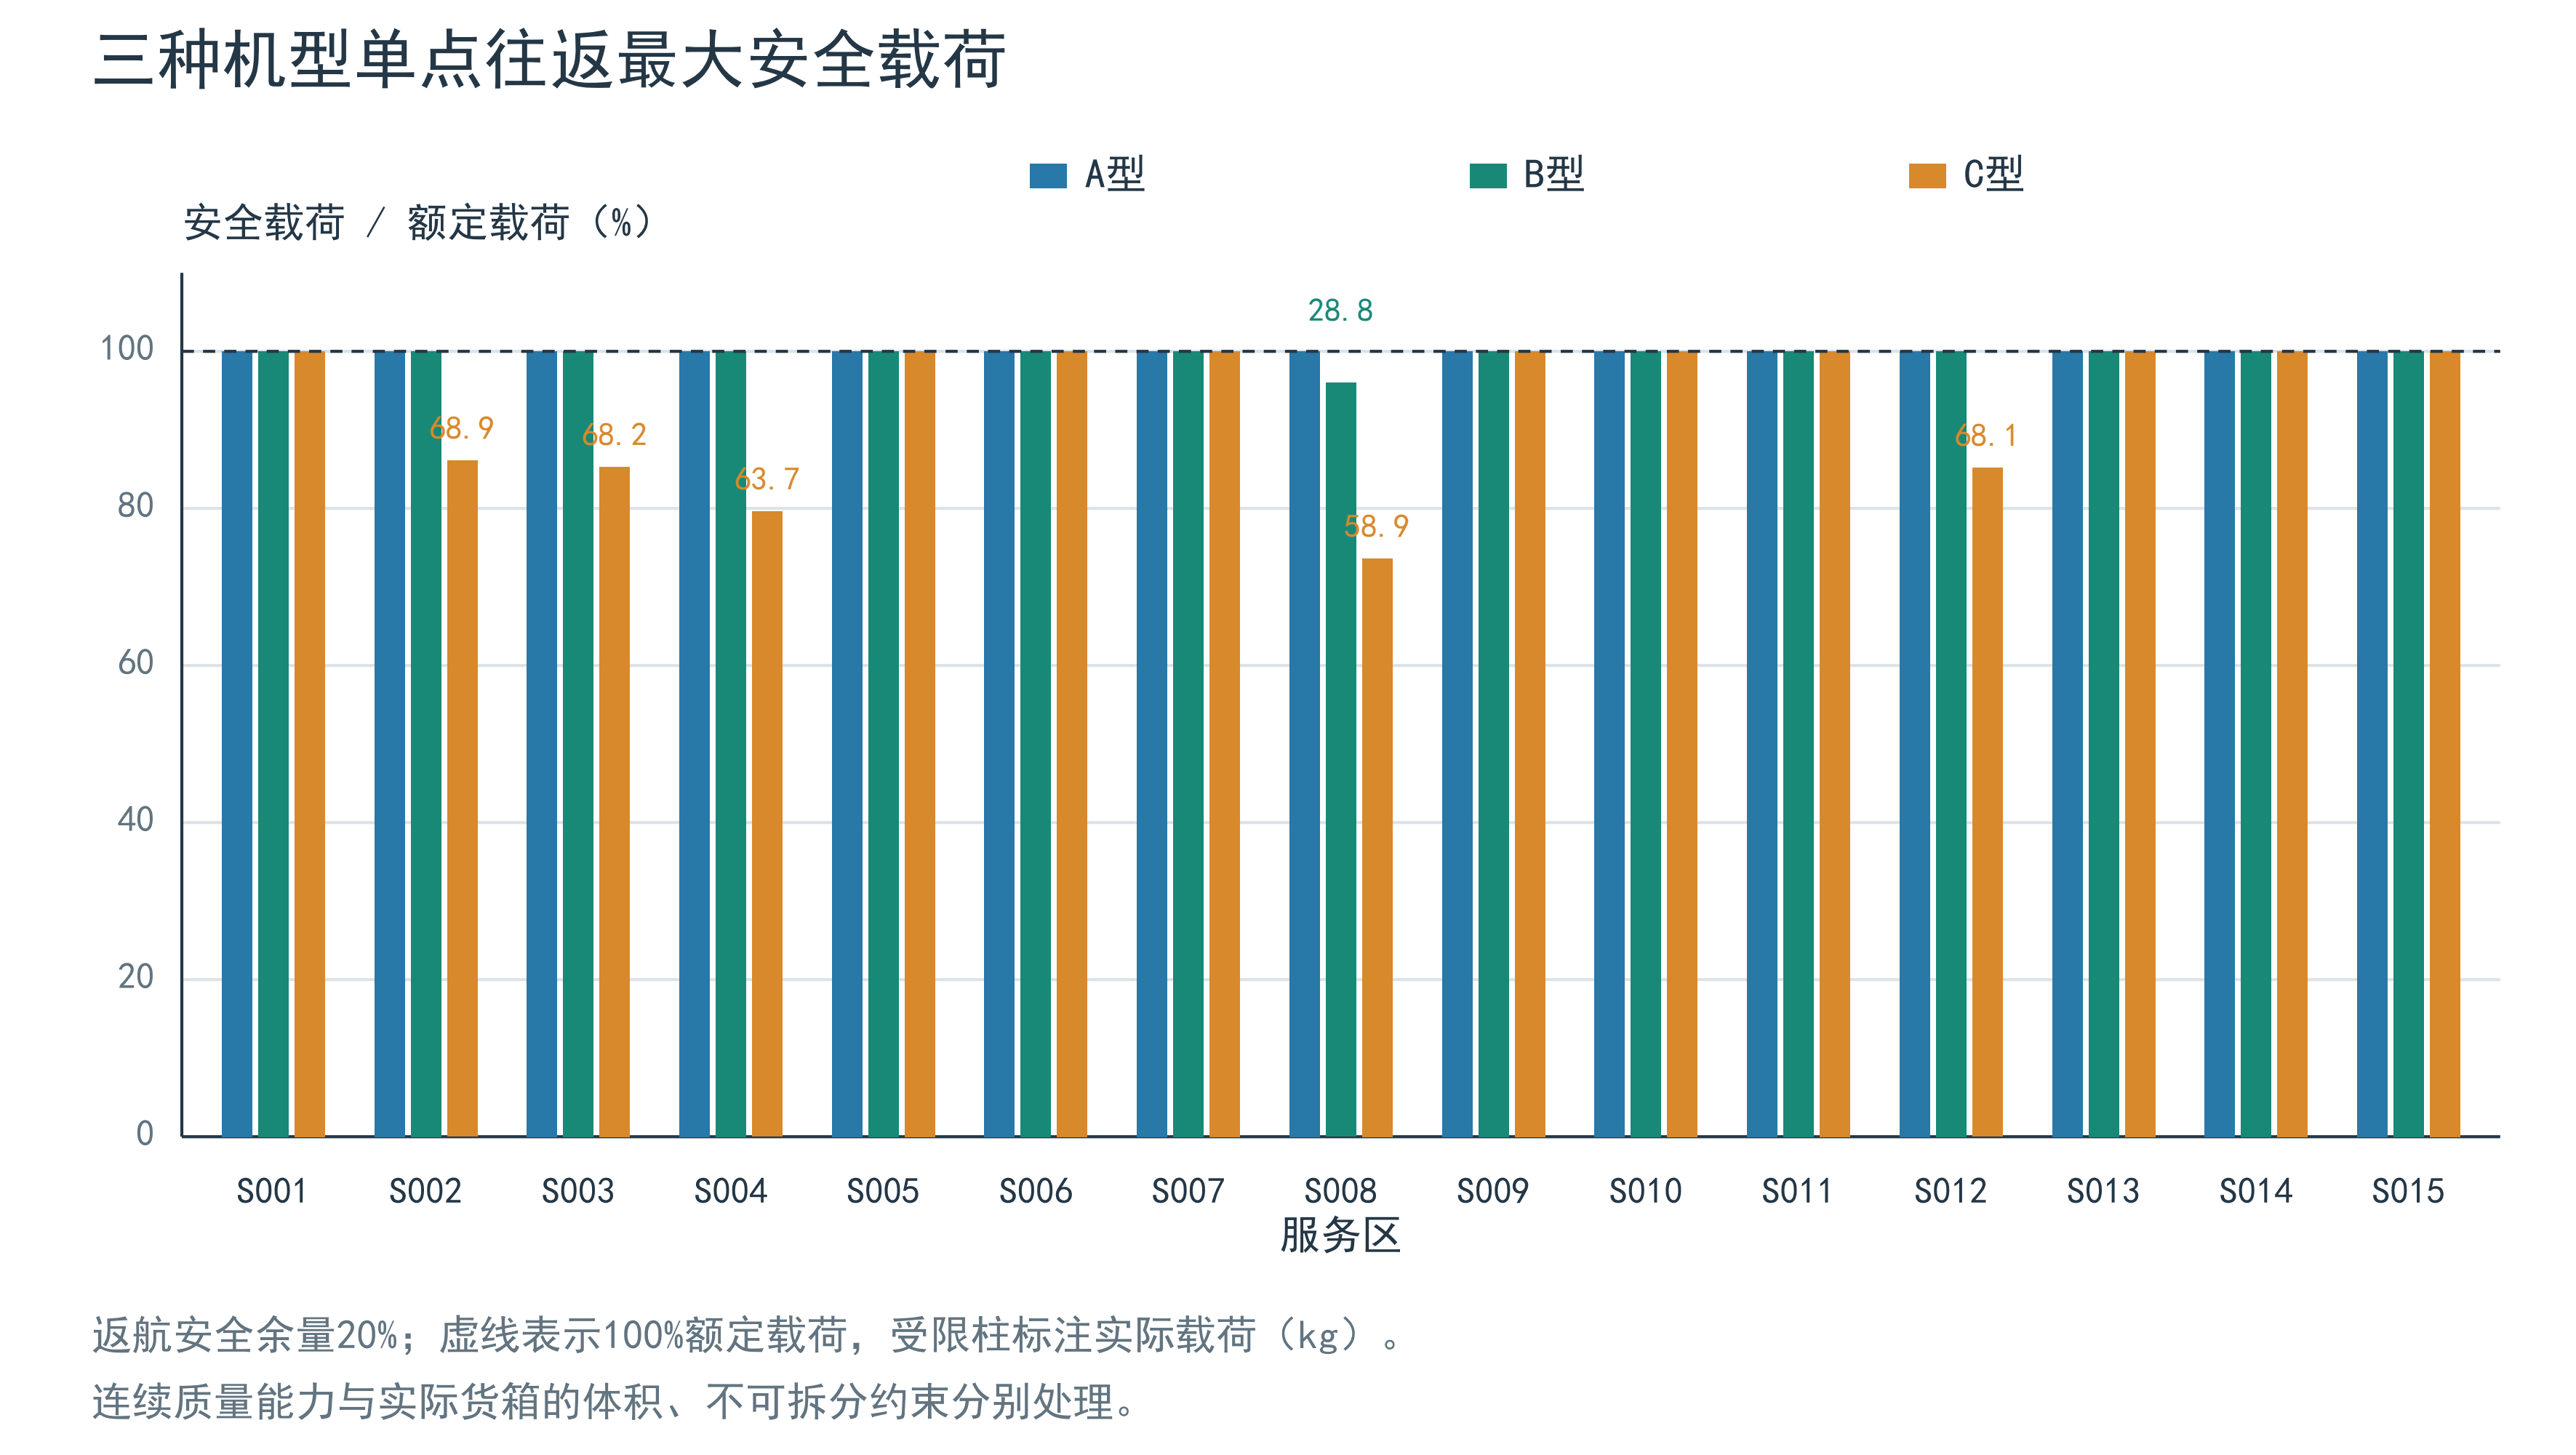
\includegraphics[width=0.95\textwidth]{pic/5.4.1.png}
    \caption{三种机型单点往返最大安全载荷占额定载荷的比例}
    \label{fig:q1_safe_payload_ratio}

    \vspace{2mm}
    \begin{minipage}{0.95\textwidth}
        \small
        注：虚线表示$100\%$额定载荷；
        受限柱上的数值为实际最大安全载荷，单位为kg。
        返航安全余量取$20\%$。
    \end{minipage}
\end{figure}

结合表~\ref{tab:q1_safe_payload}
与图~\ref{fig:q1_safe_payload_ratio}可知，
A型在全部服务区均可达到额定载质量$25\,\mathrm{kg}$，
其载荷上限由额定载质量决定。
B型仅在S008受到往返能量约束，
最大安全载荷约为$28.802\,\mathrm{kg}$，
相当于额定载质量的$96.01\%$。

C型在S002、S003、S004、S008和S012受到能量约束，
其余服务区均可达到额定载质量$80\,\mathrm{kg}$。
其中，S008对应的C型最大安全载荷最低，
约为$58.905\,\mathrm{kg}$，
仅为额定载质量的$73.63\%$，
载荷能力受限最为明显。

上述结果表明，较大的额定载质量并不意味着能够在所有航线上满载运行。
随着载荷增加，可用航程缩短，爬升能耗也随之增加；
在航段距离和地形高差共同作用下，
部分航线的往返能量约束先于额定载质量约束生效。
因此，后续货箱组批应采用各机型与服务区对应的安全载荷上限，
而不能统一按额定载质量装载。

\subsubsection{货箱组批结果}

按照式~\eqref{eq:q1_lex_objective}求解，
全部80个货箱共分为18个运输架次，
其中B型9架次、C型9架次，未选用A型。
架次摘要如表~\ref{tab:q1_batches}所示，
原始货箱编号的完整对应关系保存在结果附件中。

\begin{table}[htbp]
    \centering
    \caption{第一问基准货箱组批方案}
    \label{tab:q1_batches}
    \small
    \begin{tabular}{lllrrrr}
        \toprule
        架次 & 服务区 & 机型 & 箱数 &
        质量/kg & 体积/m$^3$ & 能耗/kWh \\
        \midrule
        P001 & S001 & C & 7 & 76 & 0.159 & 2.917477 \\
        P002 & S001 & C & 8 & 78 & 0.235 & 2.995661 \\
        P003 & S002 & B & 3 & 25 & 0.067 & 2.713386 \\
        P004 & S002 & C & 5 & 56 & 0.144 & 5.721171 \\
        P005 & S003 & B & 3 & 25 & 0.067 & 2.779588 \\
        P006 & S003 & C & 5 & 56 & 0.144 & 5.764319 \\
        P007 & S004 & C & 6 & 59 & 0.156 & 6.152871 \\
        P008 & S005 & C & 6 & 59 & 0.156 & 4.222152 \\
        P009 & S006 & C & 6 & 59 & 0.156 & 2.597321 \\
        P010 & S007 & C & 5 & 45 & 0.129 & 3.410417 \\
        P011 & S008 & C & 5 & 45 & 0.129 & 5.835969 \\
        P012 & S009 & B & 3 & 25 & 0.067 & 2.096184 \\
        P013 & S010 & B & 3 & 25 & 0.067 & 1.822820 \\
        P014 & S011 & B & 3 & 25 & 0.067 & 1.073904 \\
        P015 & S012 & B & 3 & 25 & 0.067 & 2.752261 \\
        P016 & S013 & B & 3 & 25 & 0.067 & 1.824515 \\
        P017 & S014 & B & 3 & 25 & 0.067 & 2.139813 \\
        P018 & S015 & B & 3 & 25 & 0.067 & 2.307304 \\
        \bottomrule
    \end{tabular}
\end{table}

基准方案汇总指标为
\begin{align}
    N &=18,\\
    E &=59.127133652\,\mathrm{kWh},\\
    T_{\mathrm{sum}}
      &=32775.128089\,\mathrm{s}.
\end{align}
累计作业时间约为$546.252\,\mathrm{min}$，
是各架次完整作业时间之和，不是多机并行执行的总历时。
B型和C型各9架次也不表示需要各配置9架实体无人机，
本问尚未引入实体机数量约束。

方案中最低返航SOC为$23.089108\%$，
对应S004的C型运输架次，
高于基准下限$20\%$约$3.089108$个百分点。
未选用A型是本组需求、参数与目标排序共同作用的结果，
不能据此推断A型在其他任务条件下没有使用价值。

\subsubsection{架次数下界与最优性说明}

S001的货物总质量为$154\,\mathrm{kg}$，
S002和S003均为$81\,\mathrm{kg}$。
三种机型中最大的额定载质量为$80\,\mathrm{kg}$，
因此这三个服务区均至少需要2架次。
其余12个服务区各有配送需求，至少需要1架次，
从而得到总架次数下界
\begin{equation}
    N
    \geq
    \left\lceil\frac{154}{80}\right\rceil
    +
    \left\lceil\frac{81}{80}\right\rceil
    +
    \left\lceil\frac{81}{80}\right\rceil
    +12
    =18.
\end{equation}

实际方案满足全部质量、体积和能量约束，
并达到18架次，因而第一层目标已达到该下界。
在最少架次数条件下，
完整模式枚举与动态规划进一步比较能耗和累计作业时间，
得到给定工作假设、航段数据及数值精度下的全局字典序最优方案。

该下界依赖第一问不得跨服务区组批的条件，
不能直接作为第二问多点运输的架次数下界。

\subsection{目标优先级对比}

为分析架次数、能耗与时间之间的权衡，
分别采用能耗优先和累计作业时间优先的目标排序重新求解，
结果如表~\ref{tab:q1_priority}所示。

\begin{table}[htbp]
    \centering
    \caption{不同目标优先级下的组批结果}
    \label{tab:q1_priority}
    \begin{tabular}{lrrr}
        \toprule
        字典序目标 & 架次数 & 能耗/kWh & 累计作业时间/s \\
        \midrule
        $N\rightarrow E\rightarrow T_{\mathrm{sum}}$
        &18&59.127134&32775.128089\\
        $E\rightarrow N\rightarrow T_{\mathrm{sum}}$
        &19&59.029753&34439.090232\\
        $T_{\mathrm{sum}}\rightarrow N\rightarrow E$
        &18&59.127134&32775.128089\\
        \bottomrule
    \end{tabular}
\end{table}

能耗优先方案比基准增加1架次，
总能耗减少约$0.097381\,\mathrm{kWh}$，
降幅约为$0.1647\%$，
但累计作业时间增加约$1663.962\,\mathrm{s}$，
即$27.733\,\mathrm{min}$。
累计作业时间优先方案在本数据下与基准指标相同。

因此，本算例中进一步降低能耗需要付出额外架次和作业时间代价。
基准选择架次数优先，是对减少运输任务数量的偏好，
并非认定该优先级在所有救援场景中均为唯一合理选择。

\subsection{独立核验与适用范围}

使用独立于组批求解程序的检查程序，
从原始货箱数据重新计算各架次的质量、体积、
去程载荷、空载返程能耗、返航SOC及完整作业时间。
核验结果表明，80个货箱均恰好分配一次，
目的地正确，18个架次均满足载质量、体积和返航安全余量要求，
汇总能耗与时间同求解结果一致。

上述结果依赖标准航程能量标定、爬升效率解释及
未额外计入运输交接悬停能耗等工作假设。
因此，最优性结论针对当前确定性数学模型成立，
不代表实际飞行系统在其他能耗解释或环境条件下仍具有相同最优方案。
安全余量变化下的载荷与组批重算结果将在敏感性分析部分进一步讨论。

% 导言区需包含：
% \usepackage{amsmath,amssymb,booktabs}

\section{问题二：异构无人机多点多架次调度}

问题二允许运输无人机在同一架次中访问多个服务区，
并引入实体无人机、共享电池、充电周转及物资配送时限约束。
因此，需要联合确定货箱组批、访问顺序、执行机型、
实体无人机、电池编号和任务开始时刻。

本问继承第一问的航段时间与运输能耗计算规则，
但不固定第一问的货箱组批及机型选择。
由于多点运输与有限资源调度改变了可行域，
第一问的18架次下界不能直接用于本问。

\subsection{联合调度模型}

\subsubsection{决策变量与任务表示}

设$\mathcal{B}$为全部货箱集合，
$\mathcal{U}_g$和$\mathcal{E}_g$分别为机型$g$
对应的实体无人机集合和共享电池集合。
附件给定的资源数量为
\begin{equation}
\begin{aligned}
    |\mathcal{U}_A|&=4,\quad
    |\mathcal{U}_B|=2,\quad
    |\mathcal{U}_C|=2,\\
    |\mathcal{E}_A|&=6,\quad
    |\mathcal{E}_B|=4,\quad
    |\mathcal{E}_C|=4.
\end{aligned}
\end{equation}

对运输架次$k$，主要决策包括：
货箱集合$\mathcal{B}_k$、执行机型$g_k$、
实体无人机$u_k$、电池$e_k$、
准备开始时刻$s_k$以及访问序列
\begin{equation}
    \pi_k=(i_{k1},i_{k2},\ldots,i_{km_k}),
\end{equation}
其中$m_k$为该架次的服务区访问次数。
每架次均从O01出发，并在完成交付后返回O01。

定义$x_{bk}\in\{0,1\}$表示货箱$b$是否分配给架次$k$，
则所有货箱满足
\begin{equation}
    \sum_k x_{bk}=1,
    \qquad \forall b\in\mathcal{B}.
    \label{eq:q2_box_once}
\end{equation}
同时，所分配货箱的目的地必须出现在对应架次的访问序列中，
并且只能在其正确目的地完成交付。

\subsubsection{多点运输的载荷更新}

设$\mathcal{B}_{k\ell}$为架次$k$在第$\ell$次访问时
交付的货箱集合。
各交付集合互不重叠，且满足
\begin{equation}
    \bigcup_{\ell=1}^{m_k}\mathcal{B}_{k\ell}
    =
    \mathcal{B}_k.
\end{equation}

起飞时的货物质量与体积分别为
\begin{equation}
    q_{k0}=\sum_{b\in\mathcal{B}_k}w_b,
    \qquad
    V_{k0}^{\mathrm{load}}
    =
    \sum_{b\in\mathcal{B}_k}v_b.
\end{equation}
完成第$\ell$次交付后，剩余载荷更新为
\begin{align}
    q_{k\ell}
    &=
    q_{k,\ell-1}
    -
    \sum_{b\in\mathcal{B}_{k\ell}}w_b,\\
    V_{k\ell}^{\mathrm{load}}
    &=
    V_{k,\ell-1}^{\mathrm{load}}
    -
    \sum_{b\in\mathcal{B}_{k\ell}}v_b.
\end{align}
因此，所有交付完成后应有
\begin{equation}
    q_{km_k}=0,
    \qquad
    V_{km_k}^{\mathrm{load}}=0.
\end{equation}

各航段均需满足载质量与体积限制：
\begin{equation}
    0\leq q_{k\ell}\leq Q_{g_k},
    \qquad
    0\leq V_{k\ell}^{\mathrm{load}}\leq V_{g_k}.
\end{equation}
由于本问只交付货物而不沿途取货，
载荷和体积随交付单调减少；
但在能耗计算中，仍需逐航段使用对应的实际剩余载荷。

\subsubsection{逐航段能耗与返航约束}

记$i_{k0}=i_{k,m_k+1}=0$。
架次$k$的总能耗为
\begin{equation}
    E_k
    =
    \sum_{\ell=0}^{m_k}
    E_{g_k,i_{k\ell},i_{k,\ell+1}}(q_{k\ell}),
    \label{eq:q2_sortie_energy}
\end{equation}
其中，航段能耗函数沿用公共物理模型：
\begin{equation}
    E_{gij}(q)
    =
    E_g^{\mathrm{use}}\frac{d_{ij}}{L_g(q)}
    +
    \frac{(m_g+q)g_0h_{ij}^{+}}
    {\eta_g\,3.6\times10^6}.
\end{equation}

每次服务区交付后，下一航段均从该点地面以上
$30\,\mathrm{m}$作业高度重新爬升，
再完成巡航与下降。
不能将多点访问视为全程保持固定巡航高度，
也不能用起飞载荷计算后续全部航段的能耗。

全架次返航安全约束为
\begin{equation}
    E_k
    \leq
    (1-\rho_{g_k})E_{g_k}^{\mathrm{use}},
\end{equation}
对应返航SOC为
\begin{equation}
    \sigma_k
    =
    1-\frac{E_k}{E_{g_k}^{\mathrm{use}}}
    \geq \rho_{g_k}.
\end{equation}
上述能耗表达仍依赖已说明的能量标定、
爬升效率解释及未额外计入运输交接悬停能耗等工作假设。

\subsection{任务时刻与物资时限约束}

\subsubsection{起飞、到达与交付时刻}

设架次$k$装载$n_k$个货箱，
则起飞时刻为
\begin{equation}
    t_k^{\mathrm{off}}
    =
    s_k+t_{g_k}^{\mathrm{prep}}
    +n_k t_{g_k}^{\mathrm{load}}.
\end{equation}

以$a_{k\ell}$和$c_{k\ell}$分别表示
第$\ell$次访问的到达时刻和交接完成时刻。
首个服务区的到达时刻为
\begin{equation}
    a_{k1}
    =
    t_k^{\mathrm{off}}
    +
    t_{g_k,0,i_{k1}}^{\mathrm{fly}}.
\end{equation}
之后按访问顺序递推：
\begin{align}
    c_{k\ell}
    &=
    a_{k\ell}
    +t_{g_k}^{\mathrm{base}}
    +|\mathcal{B}_{k\ell}|t_{g_k}^{\mathrm{box}},\\
    a_{k,\ell+1}
    &=
    c_{k\ell}
    +t_{g_k,i_{k\ell},i_{k,\ell+1}}^{\mathrm{fly}},
    \qquad \ell<m_k.
\end{align}

对在第$\ell$次访问时交付的货箱$b$，
其交付完成时刻为
\begin{equation}
    T_b=c_{k\ell},
    \qquad b\in\mathcal{B}_{k\ell}.
\end{equation}
全部交付完成后，返航时刻为
\begin{equation}
    f_k
    =
    c_{km_k}
    +
    t_{g_k,i_{km_k},0}^{\mathrm{fly}}.
\end{equation}

上述计算将整次交接结束作为该批货箱的完成时刻，
未将到达服务区直接等同于完成交付。

\subsubsection{硬时限与软期望时间}

设$\mathcal{B}_{\mathrm{med}}$为医疗货箱集合，
$\mathcal{B}_{\mathrm{first}}$为首批保障货箱集合，
$d_b$为期望送达时刻，$d_b^{\mathrm{first}}$为首批截止时刻。
两类硬时限分别表示为
\begin{align}
    T_b&\leq d_b,
    &&\forall b\in\mathcal{B}_{\mathrm{med}},\\
    T_b&\leq d_b^{\mathrm{first}},
    &&\forall b\in\mathcal{B}_{\mathrm{first}}.
\end{align}
若同一货箱同时具有两类标记，则两条约束同时成立。

其他物资的期望送达时间用于衡量及时性，
不直接转化为硬截止时间。
对于给定期望时间的货箱，定义延误
\begin{equation}
    \delta_b=\max\{0,T_b-d_b\},
\end{equation}
并计算加权延误
\begin{equation}
    D
    =
    \sum_{b:\,d_b\text{已给定}}
    \alpha_b\delta_b.
    \label{eq:q2_delay}
\end{equation}
其中$\alpha_b$为原始应急优先系数，
故$D$的单位为优先系数加权秒。
没有期望时间的货箱不参与该项计算，
空白时间不能当作0。
硬时限始终作为可行性约束，不通过增加延误惩罚予以放宽。

\subsection{无人机与共享电池资源约束}

\subsubsection{机型兼容与实体无人机占用}

架次的实体无人机和电池必须与所选机型一致：
\begin{equation}
    u_k\in\mathcal{U}_{g_k},
    \qquad
    e_k\in\mathcal{E}_{g_k}.
\end{equation}

实体无人机从准备开始占用至返航落地，
对应区间为
\begin{equation}
    \mathcal{I}_k^{\mathrm{body}}=[s_k,f_k).
\end{equation}
对于使用同一实体无人机的两个不同架次$k$和$k'$，
必须满足
\begin{equation}
    u_k=u_{k'}
    \ \Longrightarrow\
    \left(
    f_k\leq s_{k'}
    \ \lor\
    f_{k'}\leq s_k
    \right).
\end{equation}
下一架次仍需完整计算固定准备及装载时间，
不因连续执行而省略。

\subsubsection{电池预留、充电与复用}

电池从准备开始即被该架次预留。
设架次$k$使用电池的返航SOC为$\sigma_k$，
其充电完成时刻为
\begin{equation}
    r_k^{\mathrm{bat}}
    =
    f_k+
    \tau_{e_k}^{\mathrm{chg}}(\sigma_k),
\end{equation}
其中$\tau_{e_k}^{\mathrm{chg}}$采用题给两阶段充电模型。

该电池的完整占用区间为
\begin{equation}
    \mathcal{I}_k^{\mathrm{battery}}
    =
    [s_k,r_k^{\mathrm{bat}}).
\end{equation}
若两个架次使用同一电池，则
\begin{equation}
    e_k=e_{k'}
    \ \Longrightarrow\
    \left(
    r_k^{\mathrm{bat}}\leq s_{k'}
    \ \lor\
    r_{k'}^{\mathrm{bat}}\leq s_k
    \right).
\end{equation}

该约束同时排除了电池任务重叠、任务与充电重叠，
以及未充满就再次投入准备的情况。
所有电池初始SOC为$100\%$，
不同电池允许并行充电。
机体和电池分别记录可用时刻，
避免将返航落地误认为电池已经恢复可用。

\subsection{多目标优化模型}

在满足货箱、路线、容量、能源、硬时限和资源约束的前提下，
定义运输任务完成时间、总能耗与架次数为
\begin{align}
    C_{\max}&=\max_k f_k,\\
    E&=\sum_k E_k,\\
    N&=|\mathcal{K}|,
\end{align}
其中$\mathcal{K}$为实际执行的运输架次集合。

基准采用字典序目标
\begin{equation}
    \operatorname{lex\,min}
    \left(D,C_{\max},E,N\right).
    \label{eq:q2_objective}
\end{equation}
首先尽量减少加权延误，再比较全部运输任务的最晚返航时刻，
随后比较总能耗和架次数。
该排序是建模选择，不使用未经说明的权重将不同单位指标直接相加。

$C_{\max}$以最后一架运输无人机返回O01为准，
不是最后一个货箱的交付时刻，
也不包含最后一次返航后的补电时间。
最后补电虽不延长$C_{\max}$，仍在电池状态记录中保留。

由于货箱组批、访问顺序、离散资源选择和连续时间相互耦合，
且能耗随载荷非线性变化，
该问题具有混合离散与连续决策特征。
本研究建立上述约束与目标后，
采用启发式联合搜索获得可行调度，
不将其表述为完整混合整数非线性模型的精确求解。

% 替换位置：第6.5节起至第6章结束；整体替换原6.5--6.8
% 这是修改片段，不是完整文档；不要整份直接追加到原文末尾。
\subsection{多起点构造与模拟退火邻域搜索}
\subsubsection{初始方案与资源解码}
首先利用多起点随机扰动构造完整可行方案，再将每个架次的货箱集合、机型及批次顺序作为搜索状态。
随机性仅用于搜索，不表示需求、天气或设备状态具有随机变化。
对每个候选架次枚举所涉及服务区的访问顺序，并重新检查质量、体积、逐段载荷、能耗和硬时限。
同型号机体与电池分别维护可用时间，架次最早准备时刻为
\begin{equation}
s_k^{\mathrm{earliest}}=\max\{r_{u_k}^{\mathrm{body}},r_{e_k}^{\mathrm{battery}}\}.
\end{equation}
机体返航后恢复可用，电池返航后充电，只有充满才允许下一次准备。
候选方案改变后重新解码后续资源与任务时刻，不沿用已经失效的资源安排。

\subsubsection{邻域与候选接受}
邻域操作包括机型变更、批次插入或交换、货箱移动或交换、批次合并和拆分，
以及两个批次合并后重新分配货箱或按目的地重组。
以完成时间和延误为主的辅助评价函数驱动模拟退火，允许暂时接受部分较差候选以离开局部解；
最终保留方案仍按式~\eqref{eq:q2_objective}的字典序目标筛选。
不满足硬约束的候选不进入接受比较，不能用惩罚项放宽医疗和首批截止时间。

\subsubsection{搜索设置与范围}
在原多起点构造与局部搜索结果上，追加三轮各$180\,\mathrm{s}$的邻域搜索，
随机种子分别为20260925、20260926和20260927。
第一轮每架次最多访问3个服务区，后两轮扩大至4个。
第一轮得到25架次、$109.481\,\mathrm{min}$的候选；
第二轮得到24架次、$103.478\,\mathrm{min}$的候选；第三轮未取得实质改善。
随后将第三问联合搜索得到的运输子方案回填至第二问候选池，
在相同完成时间下进一步降低运输能耗，并重新独立核验。
访问点数上限、邻域和壁钟时间均为计算限制，不是原题约束；未穷尽全部可行调度。

\subsection{调度结果与分析}
\subsubsection{基准方案汇总}
改进方案完成80箱按期交付。16箱医疗物资与30箱首批保障物资均满足各自硬时限，
两类标记允许重叠。结果见表~\ref{tab:q2_summary}。
\begin{table}[htbp]
\centering
\small
\caption{第二问改进基准结果}
\label{tab:q2_summary}
\begin{tabular}{lr}
\toprule
指标 & 结果 \\
\midrule
交付箱数 & 80 \\
加权延误$D$ & 0 \\
运输架次数 & 24 \\
多服务区架次数 & 6 \\
最晚返航时刻/s & 6208.684865 \\
总能耗/kWh & 69.240573590 \\
实际运输机/电池数量 & 8/14 \\
最低返航SOC & $20.958111\%$ \\
最小硬时限余量/s & 194.866445 \\
\bottomrule
\end{tabular}
\end{table}
A、B、C型分别执行12、6、6架次。各实体机均执行3架次，U08的末次返航决定$C_{\max}$。
与初始基准的27架次、$117.546899\,\mathrm{min}$和$72.499522\,\mathrm{kWh}$相比，
新方案完成时间缩短$11.97\%$，能耗降低$4.50\%$。
第一问的资源与时限约束、路线限制和目标顺序均与本问不同，不能仅比较18与24架次判断优劣。
\begin{table}[htbp]
\centering
\small
\caption{改进方案的实体无人机任务分配}
\label{tab:q2_units}
\begin{tabular}{llrrr}
\toprule
无人机 & 机型 & 架次数 & 累计占用/s & 末次返航/s \\
\midrule
U01 & A & 3 & 5390.093 & 5797.832 \\
U02 & A & 3 & 5699.660 & 5817.252 \\
U03 & A & 3 & 5215.296 & 5215.296 \\
U04 & A & 3 & 5337.313 & 6113.782 \\
U05 & B & 3 & 6024.529 & 6024.529 \\
U06 & B & 3 & 5418.168 & 5418.168 \\
U07 & C & 3 & 6195.854 & 6195.854 \\
U08 & C & 3 & 6208.685 & 6208.685 \\
\bottomrule
\end{tabular}
\end{table}

\subsubsection{多点架次的载荷与时间示例}
选取C型无人机U08执行的P009架次，其使用电池C-BAT-03，携带8箱物资，路线为
\begin{equation}
\mathrm{O01}\rightarrow\mathrm{S006}\rightarrow\mathrm{S007}\rightarrow\mathrm{O01}.
\end{equation}
初始载荷$74\,\mathrm{kg}$，在S006交付4箱后降至$37\,\mathrm{kg}$，
在S007交付其余4箱后空载返回。
\begin{table}[htbp]
\centering
\small
\caption{P009架次的逐航段载荷与能耗}
\label{tab:q2_multistop}
\begin{tabular}{lrrrr}
\toprule
航段 & 载荷/kg & 起始/s & 到达/s & 能耗/kWh \\
\midrule
O01$\rightarrow$S006 & 74 & 1968.159 & 2301.527 & 2.011156 \\
S006$\rightarrow$S007 & 37 & 2625.527 & 3023.843 & 1.040271 \\
S007$\rightarrow$O01 & 0 & 3347.843 & 3907.628 & 1.438274 \\
\bottomrule
\end{tabular}
\end{table}

该架次准备开始与起飞时刻分别为$1428.158932\,\mathrm{s}$和$1968.158932\,\mathrm{s}$，
两站交付完成时刻为$2625.527260\,\mathrm{s}$和$3347.843322\,\mathrm{s}$，
均在到达之后计入完整交接时间。
全架次能耗$4.489701013\,\mathrm{kWh}$，返航SOC为$43.878737\%$。
机体于$3907.628219\,\mathrm{s}$返航，但电池到$5956.922243\,\mathrm{s}$才充满，
表明机体与能源恢复可用时间必须分别处理。

\subsection{目标优先级对比与最优性边界}
\subsubsection{目标优先级比较}
在本次搜索候选池内，分别按$D\rightarrow C_{\max}\rightarrow E\rightarrow N$
和$C_{\max}\rightarrow D\rightarrow E\rightarrow N$筛选。
以$10^{-7}\,\mathrm{s}$作为完成时间的数值比较容差，两者选中相同方案。
\begin{table}[htbp]
\centering
\small
\caption{第二问改进候选池的目标优先级比较}
\label{tab:q2_priority}
\begin{tabular}{lrrrr}
\toprule
排序 & 加权延误 & 完成时间/s & 能耗/kWh & 架次 \\
\midrule
$D\to C_{\max}\to E\to N$ & 0 & 6208.684865 & 69.240573590 & 24 \\
$C_{\max}\to D\to E\to N$ & 0 & 6208.684865 & 69.240573590 & 24 \\
\bottomrule
\end{tabular}
\end{table}

初始搜索中出现的“提前约82秒但造成普通物资延误”不再是本次最好候选之间的差异。
当前结果相同仅反映所搜索范围，不证明及时性与完成时间在全部可行方案中没有冲突。

\subsubsection{最优性边界}
由于$D\geq0$且当前方案达到$D=0$，第一层目标达到其下界；
后续完成时间、能耗与架次数没有全局最优证明。
因此本问应表述为独立验证通过的当前搜索最好可行方案，不能仅凭多轮随机搜索声称全局最优。

\subsection{独立事件回放与可行性检查}
独立程序重新读取原始货箱、设备和时限，采用40位十进制精度复算能耗与时刻，
并按准备开始、返航充电、充满恢复可用三类事件进行回放，共72个运输资源事件。
检查80箱无遗漏、无重复、无错投，质量、体积、逐段载荷、SOC及全部硬时限均合规，
机体占用和电池使用、充电、复用无冲突。
最低返航SOC为$20.958111\%$，最小硬时限余量$194.866445\,\mathrm{s}$，
最大架次能耗重算差约$4.595\times10^{-16}\,\mathrm{kWh}$。
时间、能耗、质量、体积与SOC容差分别为$10^{-7}\,\mathrm{s}$、$10^{-8}\,\mathrm{kWh}$、
$10^{-9}\,\mathrm{kg}$、$10^{-12}\,\mathrm{m^3}$及$10^{-10}$。
判定使用未舍入数据，同刻先释放后占用。
全部24架次、80箱交付和电池充电记录另附；第二问的运输验证不能替代第三问的通信检查。


\section{问题三：通信约束下运输与中继联合调度}

问题三在第二问运输调度的基础上，引入运输无人机全过程通信保障要求。
运输机在爬升、巡航、下降、交接及返航过程中，
均需与固定网关建立可用链路，或通过中继无人机完成通信。
由于链路状态随三维位置和地形遮挡变化，
运输任务的路线、执行时刻与中继位置、服务时段之间存在耦合，
因此需要联合安排运输与中继任务。

本问保留第二问的货箱、容量、能量、硬时限和资源约束，
将第二问方案作为初始候选与对照，
不预先固定其组批、路线、机型及任务开始时刻。
优化过程中同时考虑配送及时性、联合完成时间、
运输与中继总能耗及两类无人机总架次数。

\subsection{三维轨迹与通信链路模型}

\subsubsection{运输无人机全过程轨迹}

根据运输架次的实际执行时刻，
将每一航段分解为垂直爬升、水平巡航和垂直下降，
并在服务区加入交接停留阶段。
对起止时刻分别为$t_a,t_b$、
起止位置分别为$\boldsymbol{p}_a,\boldsymbol{p}_b$的运动阶段，
采用分段线性轨迹
\begin{equation}
    \boldsymbol{p}_k(t)
    =
    \boldsymbol{p}_a
    +
    \frac{t-t_a}{t_b-t_a}
    \left(\boldsymbol{p}_b-\boldsymbol{p}_a\right),
    \qquad t\in[t_a,t_b].
    \label{eq:q3_trajectory}
\end{equation}
对于交接停留阶段，
$\boldsymbol{p}_a=\boldsymbol{p}_b$，
运输机保持在服务区地面以上$30\,\mathrm{m}$的作业高度。

固定网关G01位于O01，其通信端点位置为
\begin{equation}
    \boldsymbol{p}_{G}
    =
    (x_0,y_0,z_0+h_G),
\end{equation}
其中附件给定天线离地高度$h_G=20\,\mathrm{m}$。
因此，网关通信端点不能直接放在O01地面。

全过程轨迹既用于判断服务区交接期间的通信，
也用于检查各航段的爬升、巡航和下降阶段。
仅检查服务区位置或巡航轨迹，不能代表完整运输过程的通信状态。

\subsubsection{双向链路预算}

设通信端点$u$的发射功率为$P_u^{\mathrm{tx}}$，
端点$u,v$的天线增益分别为$G_u,G_v$，
系统损耗为$L_{\mathrm{sys}}$。
端点$v$的有效接收门限由接收灵敏度与衰落裕量组成：
\begin{equation}
    P_v^{\mathrm{th}}
    =
    P_v^{\mathrm{sens}}+F_v.
\end{equation}
则方向$u\to v$允许的最大传播损耗为
\begin{equation}
    \mathcal{L}_{u\to v}^{\max}
    =
    P_u^{\mathrm{tx}}
    +G_u+G_v
    -L_{\mathrm{sys}}
    -P_v^{\mathrm{th}}.
\end{equation}

双向通信要求两个方向均可用，
因此取较严格的方向作为链路门限：
\begin{equation}
    \mathcal{L}_{uv}^{\max}
    =
    \min\left\{
    \mathcal{L}_{u\to v}^{\max},
    \mathcal{L}_{v\to u}^{\max}
    \right\}.
    \label{eq:q3_bidirectional_budget}
\end{equation}

根据附件实际参数，
载波频率为$2400\,\mathrm{MHz}$，
系统损耗为$3\,\mathrm{dB}$，
有效接收门限为
\begin{equation}
    -98+8=-90\,\mathrm{dBm}.
\end{equation}
三类双向链路允许的最大损耗如表~\ref{tab:q3_link_budget}所示。

\begin{table}[htbp]
    \centering
    \caption{双向通信链路损耗门限}
    \label{tab:q3_link_budget}
    \begin{tabular}{lc}
        \toprule
        链路类型 & 最大允许损耗/dB \\
        \midrule
        运输机—固定网关 & 122 \\
        运输机—中继接入端 & 116 \\
        中继回传端—固定网关 & 126 \\
        \bottomrule
    \end{tabular}
\end{table}

中继接入端和回传端使用不同收发参数，
不能将接入链路门限直接用于回传链路。

\subsubsection{自由空间损耗与地形遮挡}

设端点$u,v$之间的三维距离为
\begin{equation}
    d_{uv}^{\mathrm{3D}}(t)
    =
    \left\|
    \boldsymbol{p}_u(t)-\boldsymbol{p}_v(t)
    \right\|_2.
\end{equation}
将距离换算为千米后，自由空间损耗为
\begin{equation}
    \mathcal{L}_{uv}^{\mathrm{FS}}(t)
    =
    32.45
    +20\log_{10}f_{\mathrm{MHz}}
    +20\log_{10}d_{uv,\mathrm{km}}^{\mathrm{3D}}(t).
    \label{eq:q3_fspl}
\end{equation}

为判断地形遮挡，构造两端点之间的直线
\begin{equation}
    \boldsymbol{\ell}_{uv}(\theta,t)
    =
    (1-\theta)\boldsymbol{p}_u(t)
    +\theta\boldsymbol{p}_v(t),
    \qquad \theta\in[0,1].
\end{equation}
若射线经过的地形高程达到或超过对应射线高度，
则按所采用的DEM表面模型判定为存在遮挡。
定义遮挡指示量
\begin{equation}
    \chi_{uv}(t)
    =
    \begin{cases}
        1,&\text{存在地形遮挡},\\
        0,&\text{不存在地形遮挡}.
    \end{cases}
\end{equation}

按附件规定，遮挡附加损耗为$10\,\mathrm{dB}$，
故总传播损耗和链路裕量分别为
\begin{align}
    \mathcal{L}_{uv}(t)
    &=
    \mathcal{L}_{uv}^{\mathrm{FS}}(t)
    +10\chi_{uv}(t),\\
    M_{uv}(t)
    &=
    \mathcal{L}_{uv}^{\max}
    -\mathcal{L}_{uv}(t).
\end{align}
当$M_{uv}(t)\geq0$时，该双向链路可用。

由此可见，存在遮挡并不一定断联，
还需比较附加损耗后的总损耗与允许门限；
同样，不存在遮挡也不一定满足链路要求，
较大的传播距离仍可能导致损耗超限。

DEM坐标按PixelIsPoint登记方式处理。
节点表海拔与DEM高程差异保持不变，
不通过抬高节点人为消除遮挡。
在精细检查中，对射线穿越的像元以及擦边、过角位置
采用保守地形检查。

\subsection{中继任务、能耗与资源模型}

\subsubsection{悬停位置与转场剖面}

设中继架次$r$的悬停位置为
\begin{equation}
    \boldsymbol{p}_r^{\mathrm{hov}}
    =
    (x_r,y_r,z_r).
\end{equation}
悬停位置必须位于DEM覆盖范围内，
且满足附件给出的离地高度上限：
\begin{equation}
    0<
    z_r-z_{\mathrm{DEM}}(x_r,y_r)
    \leq300\,\mathrm{m}.
\end{equation}

中继从O01出发，到达悬停点后建链，
服务结束后返回O01。
沿用前述工作假设，转场海拔取
\begin{equation}
    H_r^{\mathrm{tr}}
    =
    \max\left\{
    z_r^{\mathrm{DEM,max}}+50,\,
    z_0,\,
    z_r
    \right\}.
\end{equation}
其中$z_r^{\mathrm{DEM,max}}$为O01与悬停点之间
水平航迹对应的最高地形高程。

设O01至悬停点的水平距离为$d_r$，
中继巡航、爬升和下降速度分别为
$v_R^{\mathrm{cr}}$、$v_R^{+}$和$v_R^{-}$，
则去程和返程时间分别为
\begin{align}
    t_r^{\mathrm{out}}
    &=
    \frac{H_r^{\mathrm{tr}}-z_0}{v_R^{+}}
    +\frac{d_r}{v_R^{\mathrm{cr}}}
    +\frac{H_r^{\mathrm{tr}}-z_r}{v_R^{-}},\\
    t_r^{\mathrm{back}}
    &=
    \frac{H_r^{\mathrm{tr}}-z_r}{v_R^{+}}
    +\frac{d_r}{v_R^{\mathrm{cr}}}
    +\frac{H_r^{\mathrm{tr}}-z_0}{v_R^{-}}.
\end{align}
该剖面避免悬停海拔较高时出现负爬升或负下降。

\subsubsection{有效服务时段}

设中继架次$r$的准备开始时刻为$s_r$，
固定准备时间为$t_R^{\mathrm{prep}}$，
建链时间为$t_R^{\mathrm{link}}$，
则建链完成时刻为
\begin{equation}
    c_r
    =
    s_r+t_R^{\mathrm{prep}}
    +t_r^{\mathrm{out}}
    +t_R^{\mathrm{link}}.
\end{equation}
若服务结束时刻为$e_r$，
则中继返航时刻为
\begin{equation}
    f_r=e_r+t_r^{\mathrm{back}}.
\end{equation}

中继仅在$[c_r,e_r]$内具有提供保障的资格，
到达悬停点但尚未完成建链时不能提前服务。
附件给定固定准备时间为$180\,\mathrm{s}$，
建链时间为$30\,\mathrm{s}$，
机体返航后周转时间为$300\,\mathrm{s}$。

\subsubsection{中继能耗分解}

中继计划起飞总质量采用附件值
$m_R=23.5\,\mathrm{kg}$。
其巡航功率为$1.15\,\mathrm{kW}$，
悬停功率与通信附加功率分别为
$1.05\,\mathrm{kW}$和$0.05\,\mathrm{kW}$。

水平往返能耗为
\begin{equation}
    E_r^{\mathrm{hor}}
    =
    P_R^{\mathrm{cr}}
    \frac{2d_r}{3600v_R^{\mathrm{cr}}}.
\end{equation}
爬升附加能耗为
\begin{equation}
    E_r^{\mathrm{climb}}
    =
    \frac{
    m_Rg_0
    \left[
    (H_r^{\mathrm{tr}}-z_0)
    +(H_r^{\mathrm{tr}}-z_r)
    \right]
    }{\eta_R\,3.6\times10^6}.
\end{equation}

在建链阶段按悬停功率与通信附加功率之和计耗的工作假设下，
\begin{align}
    E_r^{\mathrm{link}}
    &=
    (P_R^{\mathrm{hov}}+P_R^{\mathrm{com}})
    \frac{t_R^{\mathrm{link}}}{3600},\\
    E_r^{\mathrm{service}}
    &=
    (P_R^{\mathrm{hov}}+P_R^{\mathrm{com}})
    \frac{e_r-c_r}{3600}.
\end{align}
全架次能耗为
\begin{equation}
    E_r
    =
    E_r^{\mathrm{hor}}
    +E_r^{\mathrm{climb}}
    +E_r^{\mathrm{link}}
    +E_r^{\mathrm{service}}.
\end{equation}

中继能源组件可用能量为$3.2\,\mathrm{kWh}$，
返航SOC下限为$20\%$，因此
\begin{equation}
    E_r\leq0.8\times3.2=2.56\,\mathrm{kWh}.
\end{equation}
下降不另计附加能耗，
准备、周转阶段也不加入缺乏参数依据的额外耗电。

\subsubsection{机体与能源组件独立调度}

附件提供2架中继无人机和6组共享能源组件，
组件初始均为满电，再次使用前必须充满。
中继机体与能源组件的占用区间分别为
\begin{align}
    \mathcal{I}_r^{\mathrm{body}}
    &=
    [s_r,f_r+t_R^{\mathrm{turn}}),\\
    \mathcal{I}_r^{\mathrm{energy}}
    &=
    [s_r,f_r+\tau_r^{\mathrm{chg}}).
\end{align}
同一机体或同一组件的占用区间不得重叠。

组件返航后立即开始充电，
可与机体周转并行；
下一架次只有在机体可用且所选组件已满电时才能开始准备。
不同组件允许并行充电，
不额外引入附件未给定的单充电器限制。

\subsection{通信保障约束与联合目标}

\subsubsection{直连与中继保障选择}

对运输架次$k$在飞行和交接期间的任意时刻$t$，
定义$y_{k0}(t)$表示是否由G01直连保障，
$y_{kr}(t)$表示是否由中继架次$r$保障。
要求
\begin{equation}
    y_{k0}(t)+\sum_r y_{kr}(t)=1.
\end{equation}

采用直连优先规则：
\begin{equation}
    M_{kG}(t)\geq0
    \quad\Longrightarrow\quad
    y_{k0}(t)=1.
\end{equation}
直连不可用时，只有同时满足下列条件的中继才能被选用：
\begin{equation}
    y_{kr}(t)=1
    \quad\Longrightarrow\quad
    \begin{cases}
        c_r\leq t\leq e_r,\\
        M_{kr}^{\mathrm{access}}(t)\geq0,\\
        M_{rG}^{\mathrm{backhaul}}(t)\geq0.
    \end{cases}
    \label{eq:q3_relay_coverage}
\end{equation}
若直连与所有有效中继均不能满足条件，则该时刻发生通信中断。

本模型不允许中继之间多跳转发。
在附件未给出并发数量和切换耗时限制的情况下，
采用满足链路条件时可多机同时接入、
保障切换无额外耗时的工作假设。
该假设不代表实际带宽和网络容量已经得到验证。

上述约束描述连续时间下的通信要求，
实际求解和验证采用离散检查及局部加密，
其认证范围在后文单独说明。

\subsubsection{联合优化目标}

保留第二问的全部货箱交付、硬时限、容量、运输能量、
机体与电池资源约束，
同时加入中继飞行、能源和通信保障约束。

联合完成时间定义为
\begin{equation}
    C_{\mathrm{joint}}
    =
    \max\left\{
    \max_k f_k,\,
    \max_r f_r
    \right\}.
\end{equation}
总能耗和总架次数分别为
\begin{align}
    E_{\mathrm{total}}
    &=
    \sum_k E_k+\sum_r E_r,\\
    N_{\mathrm{total}}
    &=
    N^{\mathrm{T}}+N^{\mathrm{R}}.
\end{align}

基准采用字典序目标
\begin{equation}
    \operatorname{lex\,min}
    \left(
    D,C_{\mathrm{joint}},
    E_{\mathrm{total}},N_{\mathrm{total}}
    \right).
\end{equation}
联合完成时间包含中继最终返航，
但不包含最终补电和最终机体周转。
医疗及首批保障硬时限始终保持，
不能以延误罚项替代。

% 替换位置：第7.4节起至第7章结束；整体替换原7.4--7.6
% 这是修改片段，不是完整文档；不要整份直接追加到原文末尾。
\subsection{候选生成与联合搜索方法}
\subsubsection{空间候选与初始匹配}
初始阶段采用网格、服务区位置和地形高点生成中继候选，离地高度取150米和300米，
经DEM范围、高度及回传链路筛选后形成597个候选位置。
从原时间候选组合中提取49个位置和1904组三架次结构，重新匹配改进运输方案，
未找到满足该结构的安排。这属于有限搜索失败，不能解释为原问题不可行。

\subsubsection{通信服务日历参与运输调度}
进一步采用一架中继持续服务、另一架先后执行两个中继任务的结构，
将服务窗口、返航、机体周转、再次准备与建链时间纳入运输候选的可执行性检查。
分别以初始方案和改进第二问组批为起点，调整运输机型、批次顺序、访问顺序及准备时刻，
使需要中继的航段避开中继尚未建链或换场的时段。
三处位置沿用候选130、511和489，最终按实际通信需求重新确定服务起止时刻。
这不是固定第二问全部任务时刻后追加中继。

\subsubsection{计算限制}
服务日历搜索种子为20260928，时间预算180秒，包含最终细检查的实际耗时约182.748秒。
候选运输批次最多涉及4个服务区；中继位置与三架次结构仍受限制。
本轮服务日历搜索暂要求所有已给定期望时限均满足，以寻找$D=0$方案，
这只是搜索限制，普通物资期望时间在原模型中仍为软目标。
未穷举连续位置、任意组批和中继任务数量，也未证明全部离散候选范围内的最优性。

\subsection{联合调度结果与权衡分析}
\subsubsection{中继位置与任务安排}
改进方案使用2架中继机、3组初始满电能源组件执行3个中继架次。
三处悬停位置与初始方案相同，但服务起止、返航时刻及能耗已改变。
\begin{table}[htbp]
\centering
\small
\caption{改进方案的中继悬停位置}
\label{tab:q3_locations}
\begin{tabular}{llrrr}
\toprule
架次 & 机体 & 经度/度 & 纬度/度 & 海拔/m \\
\midrule
R001 & R01 & 109.204167 & 23.048056 & 837.268860 \\
R002 & R02 & 109.270134 & 23.015271 & 627.188568 \\
R003 & R02 & 109.266111 & 23.056389 & 623.466492 \\
\bottomrule
\end{tabular}
\end{table}
\begin{table}[htbp]
\centering
\small
\caption{改进方案的中继任务安排}
\label{tab:q3_relay_schedule}
\begin{tabular}{lrrrrr}
\toprule
架次 & 准备/s & 建链完成/s & 服务结束/s & 返航/s & 能耗/kWh \\
\midrule
R001 & 325.265 & 1056.880 & 5721.485 & 6302.231 & 1.717471 \\
R002 & 130.908 & 738.785 & 3329.431 & 3768.932 & 1.019583 \\
R003 & 4315.907 & 5077.631 & 5506.123 & 6099.161 & 0.457479 \\
\bottomrule
\end{tabular}
\end{table}

R001、R002、R003的返航SOC分别为$46.329029\%$、$68.138039\%$和$85.703779\%$。
R002于$3768.932416\,\mathrm{s}$返航，完成300秒周转后于$4068.932416\,\mathrm{s}$恢复机体可用，
早于R003的准备时刻$4315.906989\,\mathrm{s}$，两次机体占用不冲突。
但R002的能源组件到$4683.137907\,\mathrm{s}$才充满，不能直接承接R003。

\subsubsection{联合方案汇总}
80箱全部按期交付，医疗及首批硬时限全部满足，$D=0$。
\begin{table}[htbp]
\centering
\small
\caption{第三问改进联合调度结果}
\label{tab:q3_summary}
\begin{tabular}{lr}
\toprule
指标 & 结果 \\
\midrule
运输/中继架次 & 24/3 \\
运输最晚返航/s & 6208.684865 \\
联合最晚返航/s & 6302.230771 \\
运输能耗/kWh & 69.240573590 \\
中继能耗/kWh & 3.194532893 \\
总能耗/kWh & 72.435106483 \\
运输机/运输电池 & 8/14 \\
中继机/能源组件 & 2/3 \\
\bottomrule
\end{tabular}
\end{table}

联合完成时间为$105.037180\,\mathrm{min}$，由R001的最终返航决定，
比运输最晚返航晚$93.545906\,\mathrm{s}$。
相较初始联合方案，完成时间缩短$13.61\%$，总能耗降低$4.53\%$。
联合搜索得到的运输子方案同时满足第二问，并在相同完成时间下具有略低能耗，
因此回填为第二问最终候选。两问运输表相同是候选比较与回填的结果，不是事先固定的约束。

\subsubsection{目标优先级比较}
按$D\rightarrow C_{\mathrm{joint}}\rightarrow E_{\mathrm{total}}\rightarrow N_{\mathrm{total}}$
与$C_{\mathrm{joint}}\rightarrow D\rightarrow E_{\mathrm{total}}\rightarrow N_{\mathrm{total}}$
筛选当前候选池，均选中上述$D=0$、$6302.230771\,\mathrm{s}$、
$72.435106483\,\mathrm{kWh}$及24运输加3中继架次的方案。
这不证明两个完整优化问题具有相同的全局最优解，尤其本轮服务日历搜索偏重全部按期交付的候选。

\subsection{独立轨迹回放与通信验证}
\subsubsection{任务与资源检查}
独立程序重读原始货箱、设备、通信参数和DEM，重构运输全过程轨迹，复算中继飞行与能耗，
检查所有机体、运输电池及中继组件的占用、周转和充电。
两种优先级选中的方案均通过检查，运输最低返航SOC为$20.958111\%$，
最小硬时限余量为$194.866445\,\mathrm{s}$。

\subsubsection{分辨率加密检查}
检查覆盖爬升、巡航、下降、交接以及中继建链与服务边界，结果见表~\ref{tab:q3_refinement}。
\begin{table}[htbp]
\centering
\small
\caption{改进方案的通信分辨率核验}
\label{tab:q3_refinement}
\begin{tabular}{lrrr}
\toprule
时间步长与空间检查 & 点数 & 失败点 & 最小裕量/dB \\
\midrule
1秒，5米射线 & 36218 & 0 & 0.000703269 \\
0.5秒，2.5米射线 & 72113 & 0 & 0.000356918 \\
0.5秒及局部加密，全穿越像元 & 73220 & 0 & 0.000155292 \\
\bottomrule
\end{tabular}
\end{table}

对端点裕量低于$0.02\,\mathrm{dB}$或保障源变化的区间细化至不超过0.05秒，
对定位到的切换点二分至$10^{-7}\,\mathrm{s}$。
最差所选链路裕量出现在P010巡航阶段$t=3860.254957\,\mathrm{s}$附近。

\subsubsection{验证结论与适用范围}
准确结论为：\textbf{在所述时空分辨率下未发现中断}。
离散检查未严格排除采样间隙中的短暂失效，不能写成已数学证明中断时长为零。
全部196个运输阶段保守列入尚未严格认证区间；248条通信保障记录及其任务关联用于第四问冻结。
第一层$D=0$达到非负下界，后续目标无全局最优证明。
标准航程能量标定、爬升效率解释、未计运输交接悬停能耗，
以及中继多机并发与零额外切换耗时仍是需要用户核验的工作假设。


\section{问题四：救援任务分区与资源配置优化}

\subsection{问题分析与建模思路}

问题四要求在第三问调度方案保持不变的条件下，将15个服务区分别划分为
$K=2$和$K=3$个任务组，并确定各组独立执行运输与通信保障任务所需的资源配置。
与前两问的调度优化不同，本问不再调整货箱组批、访问顺序及任务时刻，
而是研究资源由集中共享转为分组独立使用后产生的额外配置和库存缺口。

本问的主要困难在于：运输架次可能同时访问多个服务区，
使服务区之间形成不可拆分的绑定关系；中继架次可能为多个任务组提供保障，
需要明确其独立执行方式；电池和能源组件的复用还受到充电时间约束，
不能直接将第三问使用的不同编号数量视为最小配置。

为此，本文首先构造必须同组的服务区块，
再通过固定时序下的区间重叠计算各组最小资源需求，
最后完整枚举合法分区，按资源缺口、配置规模和工作量均衡性进行字典序优化。

\subsection{冻结方案与解释口径}

\subsubsection{冻结调度的定义}

以第三问基准方案作为冻结输入，保持以下内容不变：
运输货箱及其目的地、架次访问顺序、运输机型、
准备与起飞时刻、交付完成与返航时刻，
以及中继位置、建链与服务时段、返航时刻和实际通信保障关系。

冻结并不要求所有资源承接编号保持不变。
本文基准允许组内同型号资源重新编号，
但不得因此改变任务内容、物理轨迹或执行时序。

设冻结运输架次集合为$\mathcal{T}$，
原中继架次集合为$\mathcal{R}$，
服务区集合为
\begin{equation}
\mathcal{V}=\{\mathrm{S001},\ldots,\mathrm{S015}\}.
\end{equation}
分区后，每个服务区恰好属于一个非空任务组，
各组在任务执行期间不得相互借用机体、电池或能源组件。

\subsubsection{跨组中继与资源编号假设}

由于原文未明确跨组中继的独立执行方式以及资源编号是否必须保留，
本文采用以下基准解释，
均属于\textbf{工作假设，需要用户核验}：

\begin{enumerate}
    \item 允许组内同型号机体、电池及能源组件重新编号和合法复用，
    仅改变资源承接关系，不改变任何任务时刻。

    \item 当一个冻结中继架次实际保障多个任务组时，
    各相关组分别配置该架次的完整任务副本。
    每个副本保留原准备、转场、建链、服务、返航和周转过程，
    并独立计入资源占用与能耗。

    \item 同一组内对同一原中继架次的多次引用只计一个副本，
    不同组的副本由独立资源执行。

    \item 能源组件返航后立即充电，充电可与中继机体周转并行；
    不增加附件未规定的充电器数量或准备工位限制。
\end{enumerate}

本文同时比较禁止复制中继架次、继承原实体编号两种替代解释。
不额外施加地理连通、服务区数量相等或空间紧凑等约束。

\subsection{必须同组关系与分区变量}

设$\mathcal{V}_k$为运输架次$k$访问的服务区集合。
由于同一运输架次不能拆分到不同任务组，
对任意$i,j\in\mathcal{V}_k$均有
\begin{equation}
\operatorname{group}(i)=\operatorname{group}(j).
\end{equation}

将共同出现在一个运输架次中的服务区连接，
通过并查集求取传递闭包。
实际计算得到14个不可拆分服务区块：
$\{\mathrm{S011},\mathrm{S012}\}$构成一个块，
其余13个服务区分别构成单点块。

记块集合为$\mathcal{B}$，定义二元变量
\begin{equation}
z_{a\ell}=
\begin{cases}
1, & \text{服务区块$a$分配至任务组$\ell$},\\
0, & \text{否则},
\end{cases}
\qquad
a\in\mathcal{B},\quad \ell=1,\ldots,K.
\end{equation}

分区约束为
\begin{align}
\sum_{\ell=1}^{K}z_{a\ell}&=1,
&& a\in\mathcal{B},\\
\sum_{a\in\mathcal{B}}z_{a\ell}&\geq 1,
&& \ell=1,\ldots,K.
\end{align}

由于同一运输架次访问的全部服务区已合并至同一块，
上述约束能够保证运输任务完整归属。

设$a(k)$为运输架次$k$所属的服务区块，
$\mathcal{H}_r$为原中继架次$r$实际保障的运输架次集合。
定义$c_{r\ell}$表示任务组$\ell$是否需要中继$r$的完整副本，
则
\begin{align}
c_{r\ell}&\geq z_{a(k)\ell},
&& k\in\mathcal{H}_r,\\
c_{r\ell}&\leq
\sum_{k\in\mathcal{H}_r}z_{a(k)\ell},
&& c_{r\ell}\in\{0,1\}.
\end{align}

其中，$\mathcal{H}_r$由第三问实际通信保障区间确定，
不以地理上可能覆盖的服务区替代实际保障关系。

\subsection{固定时序下的最小资源配置}

\subsubsection{资源占用区间}

本文考虑八类资源，其排列顺序为
\begin{equation}
\boldsymbol{R}=
\left(
R_{\mathrm{A机}},R_{\mathrm{B机}},R_{\mathrm{C机}},
R_{\mathrm{A电}},R_{\mathrm{B电}},R_{\mathrm{C电}},
R_{\mathrm{中继机}},R_{\mathrm{组件}}
\right).
\end{equation}
对应库存为
\begin{equation}
\boldsymbol{I}=(4,2,2,6,4,4,2,6).
\end{equation}

设运输架次$k$的准备开始和返航时刻分别为$s_k$和$f_k$，
返航SOC为$\sigma_k$。
设中继架次$r$的相应时刻为$s_r$、$f_r$，
返航SOC为$\sigma_r$，机体周转时间为$\tau^{\mathrm{turn}}=300\,\mathrm{s}$。
四类占用区间定义为
\begin{align}
\mathcal{I}^{\mathrm{T机}}_k
&=[s_k,f_k),\\
\mathcal{I}^{\mathrm{T电}}_k
&=[s_k,f_k+t^{\mathrm{ch}}_k(\sigma_k)),\\
\mathcal{I}^{\mathrm{R机}}_r
&=[s_r,f_r+\tau^{\mathrm{turn}}),\\
\mathcal{I}^{\mathrm{R能}}_r
&=[s_r,f_r+t^{\mathrm{ch}}_r(\sigma_r)).
\end{align}

充电时间沿用附件给出的两阶段模型：
\begin{equation}
t^{\mathrm{ch}}(\sigma)=
\begin{cases}
T^{\mathrm{full}}
\left[
0.65\dfrac{0.9-\sigma}{0.9}+0.35
\right],
&0\leq \sigma<0.9,\\[2mm]
T^{\mathrm{full}}\times0.35
\dfrac{1-\sigma}{0.1},
&0.9\leq \sigma\leq1.
\end{cases}
\end{equation}

全部区间采用半开形式，同一时刻先释放资源、后开始新的占用。
能源区间延伸至恢复满电，确保复用前满足满电要求。
最后一次返航后的充电不计入联合任务完成时间，
但保留在能源恢复记录中。

\subsubsection{峰值需求与具体资源分配}

记$\mathcal{J}_{\ell\gamma}$为任务组$\ell$中占用资源类型$\gamma$的任务集合，
任务$j$的占用区间为$[a_j,b_j)$。
该组该类型资源的最小配置为
\begin{equation}
n_{\ell\gamma}
=
\max_t
\sum_{j\in\mathcal{J}_{\ell\gamma}}
\mathbf{1}\{a_j\leq t<b_j\}.
\label{eq:q4_peak}
\end{equation}

式\eqref{eq:q4_peak}具有下界与可实现性两方面依据。
任意时刻同时占用的任务必须由不同实体承担，
因此最大重叠数构成资源需求下界。
另一方面，将任务按开始时刻排序，
优先复用已经释放的资源，
仅在所有已有资源均被占用时增加编号，
即可构造恰好达到最大重叠数的资源分配。

该结论成立的前提是同类型资源可互换、
所有任务从O01出发并返回O01，
且不存在额外的兼容性或转场约束。
不同机型电池分别计算，不允许混用。

未分区情况下重新计算得到最小配置
\begin{equation}
\boldsymbol{R}^{0}=(4,2,2,6,4,4,2,2).
\end{equation}

其中，中继能源组件最少需要2组。
原中继架次R002的组件于$2745.256\,\mathrm{s}$充满，
早于R003的准备开始时刻$3397.063\,\mathrm{s}$，
因此二者可以复用同一组件。
第三问使用3个不同组件编号，
并不意味着冻结时序下最少需要3组组件。

\subsection{分区优化目标}

\subsubsection{需求、缺口与库存剩余}

对资源类型$\gamma$，定义总需求、缺口及库存剩余为
\begin{align}
R_\gamma&=\sum_{\ell=1}^{K}n_{\ell\gamma},\\
\Delta_\gamma&=\max\{0,R_\gamma-I_\gamma\},\\
U_\gamma&=\max\{0,I_\gamma-R_\gamma\}.
\end{align}

各类型缺口分别报告，不允许用某类资源的富余抵消另一类短缺。
由于本问需要分析资源缺口，
库存不足的分区仍参与比较，
但须明确其执行依赖于补充相应资源。

无采购价格数据时，采用归一化缺口与配置规模：
\begin{align}
G&=\sum_{\gamma}\frac{\Delta_\gamma}{I_\gamma},\\
S&=\sum_{\gamma}\frac{R_\gamma}{I_\gamma}.
\end{align}
两者均为无量纲比较指标，
表示八类资源等权归一化后的缺口和规模，
不解释为实际经济成本。

\subsubsection{工作量与字典序目标}

定义任务组$\ell$的工作量为机体占用时间总和：
\begin{equation}
W_\ell
=
\sum_{k\in\mathcal{T}_\ell}(f_k-s_k)
+
\sum_{r\in\mathcal{R}}
c_{r\ell}(f_r+\tau^{\mathrm{turn}}-s_r).
\end{equation}
该指标包括中继周转，不包括电池充电。

以工作量变异系数衡量组间不均衡：
\begin{equation}
\mathrm{CV}
=
\frac{
\sqrt{\dfrac{1}{K}\sum_{\ell=1}^{K}(W_\ell-\overline{W})^2}
}{\overline{W}},
\qquad
\overline{W}=\frac{1}{K}\sum_{\ell=1}^{K}W_\ell.
\end{equation}

基准采用字典序目标
\begin{equation}
\operatorname{lexmin}(G,S,\mathrm{CV}).
\end{equation}
即先减少库存缺口，再控制配置规模，
最后在前两层目标最优的方案中改善工作量均衡。
该优先级属于建模选择。

\subsection{求解方法与最优性范围}

对于14个不可拆分块，
采用无标签非空分区枚举，消除组编号置换造成的重复。
两种分组数量分别为
\begin{align}
\left\{\begin{matrix}14\\2\end{matrix}\right\}
&=8191,\\
\left\{\begin{matrix}14\\3\end{matrix}\right\}
&=788970,
\end{align}
其中大括号表示第二类Stirling数。

首先缓存全部$2^{14}-1=16383$个非空块子集的资源需求与工作量，
再组合得到各合法分区的目标值。
由于库存分母均为2、4或6，
采用$12G$和$12S$进行整数比较；
工作量均衡层以$\mathrm{CV}^2$比较，
并列判断容差为$10^{-12}$。

求解完整检查了全部合法分区，
未截断候选集合，也未因时间限制提前终止。
主模型运行时间约为$3.13\,\mathrm{s}$，
两种基准在上述容差下均得到唯一最优分区。

因此，本文所述最优性仅针对
\textbf{冻结的第三问方案、所采用的中继复制和资源编号口径、
目标优先级及数值容差}。
该结论不能扩展为原始运输、通信与分区联合问题的全局最优。

\subsection{分区与配置结果}

\subsubsection{两组分区结果}

当$K=2$时，最优分区为
\begin{align}
\mathcal{V}_1&=\{\mathrm{S001}\},\\
\mathcal{V}_2&=\mathcal{V}\setminus\{\mathrm{S001}\}.
\end{align}

各组资源配置为
\begin{align}
\boldsymbol{n}_1&=(0,0,1,0,0,2,0,0),\\
\boldsymbol{n}_2&=(4,2,2,6,4,3,2,2).
\end{align}
总需求为
\begin{equation}
\boldsymbol{R}^{(2)}=(4,2,3,6,4,5,2,2).
\end{equation}

该方案缺少1架C型运输无人机和1组C型电池，
中继能源组件剩余4组，其余类型无缺口。
目标值为
\begin{equation}
G^{(2)}=0.75,\qquad
S^{(2)}=8.083333,\qquad
\mathrm{CV}^{(2)}=0.894564.
\end{equation}

两组分别承担15箱和65箱物资，
运输质量分别为154\,kg和604\,kg，
执行2个和25个运输架次。
第一组不需要中继，
第二组执行原有3个中继架次，
未产生额外中继任务副本。

\subsubsection{三组分区结果}

当$K=3$时，最优分区为
\begin{align}
\mathcal{V}_1&=\{\mathrm{S001},\mathrm{S004}\},\\
\mathcal{V}_3&=\{\mathrm{S008}\},\\
\mathcal{V}_2&=\mathcal{V}
\setminus\{\mathrm{S001},\mathrm{S004},\mathrm{S008}\}.
\end{align}

各组资源配置为
\begin{align}
\boldsymbol{n}_1&=(0,0,1,0,0,2,1,1),\\
\boldsymbol{n}_2&=(4,2,1,6,4,1,2,2),\\
\boldsymbol{n}_3&=(0,0,1,0,0,1,1,1).
\end{align}
总需求为
\begin{equation}
\boldsymbol{R}^{(3)}=(4,2,3,6,4,4,4,4).
\end{equation}

该方案缺少1架C型运输无人机和2架中继无人机，
中继能源组件剩余2组。
目标值为
\begin{equation}
G^{(3)}=1.50,\qquad
S^{(3)}=9.166667,\qquad
\mathrm{CV}^{(3)}=0.866840.
\end{equation}

三个组分别执行3、23和1个运输架次，
对应1、3和1个中继任务。
其中，第一组需要原R003的完整副本，
第三组需要原R001的完整副本，
第二组仍需要原有三个中继架次，
因而中继任务总数由3次增加至5次。

\begin{table}[htbp]
\centering
\caption{两种基准分区的资源需求与库存缺口}
\label{tab:q4_resources}
\begin{tabular}{lrrrrr}
\toprule
资源类型 & 库存 & 两组需求 & 两组缺口 & 三组需求 & 三组缺口\\
\midrule
A型运输机 &4&4&0&4&0\\
B型运输机 &2&2&0&2&0\\
C型运输机 &2&3&1&3&1\\
A型电池   &6&6&0&6&0\\
B型电池   &4&4&0&4&0\\
C型电池   &4&5&1&4&0\\
中继无人机 &2&2&0&4&2\\
中继能源组件 &6&2&0&4&0\\
\bottomrule
\end{tabular}
\end{table}

\begin{table}[htbp]
\centering
\caption{各组任务规模与机体占用工作量}
\label{tab:q4_workload}
\small
\begin{tabular}{ccrrrrrr}
\toprule
$K$ & 组别 & 箱数 & 质量/kg & 体积/$\mathrm{m}^3$
& 运输架次 & 中继任务 & 工作量/s\\
\midrule
2&1&15&154&0.394&2&0&3186.318\\
2&2&65&604&1.617&25&3&57254.225\\
\midrule
3&1&21&213&0.550&3&1&8575.845\\
3&2&54&500&1.332&23&3&52753.466\\
3&3&5&45&0.129&1&1&9781.528\\
\bottomrule
\end{tabular}
\end{table}

\subsection{资源缺口与额外配置的来源}

\subsubsection{独立配置造成的错峰复用损失}

两组方案中，第一组至少需要1架C型运输机，
第二组在$1560.159\,\mathrm{s}$由P002和P009同时占用C型机，
至少需要2架，故独立配置总数为3架。

第一组在$1907.490\,\mathrm{s}$，
P001的电池尚未恢复可用，P011已经开始占用电池，
因此至少需要2组C型电池。
第二组在$3533.649\,\mathrm{s}$，
P002、P009和P014的电池占用区间重叠，
至少需要3组。
两组独立保有后总需求为5组，高于库存4组。

这些组内峰值不必在同一时刻发生。
由于禁止跨组调配，不能以未分区的全局同时占用数
代替各组峰值之和。

三组方案中，每组均至少需要1架C型运输机，
总需求仍为3架。
第一组和第三组各需要1架中继机，
第二组需要2架，
因此中继机总需求达到4架。

\subsubsection{库存剩余、额外配置与任务重复}

为避免将不同含义混称为资源冗余，分别定义：

\begin{enumerate}
    \item 库存剩余：
    $U_\gamma=\max(0,I_\gamma-R_\gamma)$。

    \item 分区额外配置：
    \begin{equation}
    A_\gamma=R_\gamma-R_\gamma^0,
    \end{equation}
    其中$R_\gamma^0$是在相同编号口径下、
    未分区且资源可共享时的最小需求。

    \item 中继任务重复：
    由跨组完整复制产生的新增中继架次、占用时间及能耗。
\end{enumerate}

两组方案相较未分区基线，
增加1架C型运输机和1组C型电池，
未增加中继架次与能耗。

三组方案增加1架C型运输机、2架中继机和2组中继能源组件。
其中组件需求为4组，仍低于库存6组，
因此增加组件配置不等于出现组件库存缺口。

三组方案额外复制R001和R003，
增加2个中继架次，
新增能耗为
\begin{equation}
E_{\mathrm{copy}}
=
2.116178370+0.764628548
=
2.880806918\,\mathrm{kWh}.
\end{equation}
对应增加中继机体占用时间$10670.297\,\mathrm{s}$，
增加能源组件占用时间$12240.624\,\mathrm{s}$。

两种分区的运输任务均保持不变，
故加权延误仍为$D=0$，
联合完成时间均为
\begin{equation}
C_{\mathrm{joint}}=7295.419515\,\mathrm{s}.
\end{equation}
两组和三组的运输与中继总能耗分别为
\begin{align}
E_{\mathrm{total}}^{(2)}
&=75.869829\,\mathrm{kWh},\\
E_{\mathrm{total}}^{(3)}
&=78.750636\,\mathrm{kWh}.
\end{align}

\subsection{目标优先级与解释口径比较}

\subsubsection{资源配置与工作量均衡的权衡}

将目标改为
$\operatorname{lexmin}(G,\mathrm{CV},S)$后，
两种$K$均得到与基准相同的分区。
但若将均衡置于首位，
即采用$\operatorname{lexmin}(\mathrm{CV},G,S)$，
则能够显著降低组间工作量差异，
同时增加资源需求。

\begin{table}[htbp]
\centering
\caption{不同目标优先级的比较}
\label{tab:q4_priority}
\begin{tabular}{clrrr}
\toprule
$K$ & 目标优先级 & $G$ & $S$ & $\mathrm{CV}$\\
\midrule
2 & $G\rightarrow S\rightarrow\mathrm{CV}$
  &0.750000&8.083333&0.894564\\
2 & $G\rightarrow\mathrm{CV}\rightarrow S$
  &0.750000&8.083333&0.894564\\
2 & $\mathrm{CV}\rightarrow G\rightarrow S$
  &4.166667&11.833333&0.000011\\
\midrule
3 & $G\rightarrow S\rightarrow\mathrm{CV}$
  &1.500000&9.166667&0.866840\\
3 & $G\rightarrow\mathrm{CV}\rightarrow S$
  &1.500000&9.166667&0.866840\\
3 & $\mathrm{CV}\rightarrow G\rightarrow S$
  &4.333333&12.333333&0.000336\\
\bottomrule
\end{tabular}
\end{table}

基准方案优先控制资源缺口，
因此保留了明显的大组与小组差异。
均衡优先方案的$\mathrm{CV}$接近零，
但归一化缺口显著上升。
因此，资源优先方案不能被解释为所有指标均最优。

\subsubsection{禁止复制中继架次}

若禁止复制中继架次，
则同一中继架次实际保障的运输任务也必须属于同组。
在运输绑定基础上继续合并，得到三个不可拆分集合：
\begin{align}
\mathcal{C}_1&=\{\mathrm{S001}\},\\
\mathcal{C}_2&=\{\mathrm{S006}\},\\
\mathcal{C}_3&=\mathcal{V}
\setminus\{\mathrm{S001},\mathrm{S006}\}.
\end{align}

此时，$K=2$仍有3个合法无标签分区，
$K=3$仅有1个合法分区，
因此禁止复制并不导致不存在合法分组。

两组最优结果与基准一致。
三组资源需求变为
\begin{equation}
\boldsymbol{R}^{(3)}_{\mathrm{no\ copy}}
=(6,3,3,8,5,5,2,2),
\end{equation}
归一化缺口为$G=2.333333$。
该解释避免了新增中继任务，
却增加了运输机和电池的独立配置需求。

\subsubsection{继承第三问原实体编号}

若要求继承原编号，
按每组使用的不同原编号数量核算配置。
同一原编号出现在不同组时，
必须分别配置实体，不得跨组共享。

固定基准分区，仅改变编号口径，
两组和三组的需求分别为
\begin{align}
\boldsymbol{R}^{(2)}_{\mathrm{fixed,ID}}
&=(4,2,4,6,4,5,2,3),\\
\boldsymbol{R}^{(3)}_{\mathrm{fixed,ID}}
&=(4,2,5,6,4,4,4,5).
\end{align}
对应$G$分别为1.25和2.50。

若在继承编号口径下重新优化分区，
则需求分别为
\begin{align}
\boldsymbol{R}^{(2)}_{\mathrm{ID,opt}}
&=(4,2,3,6,4,4,3,4),\\
\boldsymbol{R}^{(3)}_{\mathrm{ID,opt}}
&=(5,2,3,7,4,5,4,5),
\end{align}
对应$G$分别为1.00和2.166667。

固定分区比较用于衡量重新编号的影响，
重新优化结果则反映该解释下的最优分区。
两类比较的分区条件不同，不能混为同一项收益。

\subsection{独立事件回放与结果有效性}

建立不导入分区优化器的独立检查程序，
从原始货箱和设备参数重新计算能耗、SOC、充电及周转时间，
并对导出的组内资源分配进行确定性事件回放。

独立检查确认：

\begin{enumerate}
    \item 15个服务区无遗漏、无重复，各任务组非空，
    同一运输架次涉及的服务区均属于同组。

    \item 80箱物资的归属与交付时刻保持不变，
    16箱医疗物资和30箱首批保障物资的硬时限全部满足；
    两类标记允许重叠，最小硬时限余量为
    $2082.852950\,\mathrm{s}$。

    \item 冻结任务的路线、机型、位置和各阶段时刻一致，
    249条通信保障区间完整继承，
    中继副本未被裁剪或重复计数。

    \item 组内机体与能源分配无重叠，
    能源复用前恢复满电，
    实体编号不跨组共享。

    \item 独立计算的资源峰值、配置数量、库存缺口、
    工作量和能耗与导出结果一致。

    \item 全部冻结输入的SHA-256在运行前后保持一致。
\end{enumerate}

共16个导出方案通过独立检查。
另采用受限增长分组枚举和时间占用矩阵，
重新核验全部8191个两组分区与788970个三组分区，
相应最优目标与主程序一致。

可行性判断使用未四舍五入数据。
时间、能量、SOC、质量和体积复算容差分别为
$10^{-7}\,\mathrm{s}$、
$10^{-8}\,\mathrm{kWh}$、
$10^{-10}$、
$10^{-9}\,\mathrm{kg}$和
$10^{-12}\,\mathrm{m}^3$。
资源区间按原始端点和半开规则处理，
不通过展示舍入减少资源需求。

需要强调，检查通过表示在所列资源配置下能够承接冻结任务，
不表示现有库存足够。
完整枚举表明，在基准解释下，
两种$K$均不存在完全满足现有库存的分区。

通信结论仅继承第三问的
\textbf{“在所述时空分辨率下未发现中断”}，
不构成连续通信的数学证明。
相同位置与时段的中继副本可以复用原链路几何检查，
但真实网络并发容量、共址干扰和空域运行条件尚未建模。

\subsection{结果分析}

在资源缺口与配置规模优先的条件下，
两组方案的$G$、$S$和总能耗均低于三组方案，
且无需复制中继任务，适合资源补充能力有限的情形。
三组方案不需要增加C型电池，
工作量变异系数略低，
但需要额外配置2架中继机，
并增加$2.880807\,\mathrm{kWh}$中继能耗。

分区成本主要来自组间资源共享被禁止后失去错峰复用机会，
以及跨组通信保障对应的完整中继任务复制。
上述结论依赖于冻结的第三问基准方案、
组内允许重新编号及跨组中继完整复制等解释。
若允许重新优化第三问任务时序，
资源需求可能进一步降低，
但已超出本问冻结调度下的研究范围。

\section{模型评价}

这里是模型评价



%参考文献   手工录入
%\begin{thebibliography}{9}%宽度9
% \bibitem{bib:one} ....
% \bibitem{bib:two} ....
%\end{thebibliography}

%采用bibtex方案
\cite{mittelbach_latex_2004,wright_latex3_2009,beeton_unicode_2008,vieth_experiences_2009}

\bibliographystyle{gmcm}
\bibliography{reference}


\clearpage
%附录
\begin{appendices}
%\setcounter{page}{1} %如果需要可以自行重置页码。
\section{MATLAB 源程序}
\renewcommand{\thesubsection}{A\thinskip.\thinskip\arabic{subsection}}
\subsection{第1问程序}
\vspace{-2ex}

\begin{Matlab}{code.m}
clear all
kk=2;
[mdd,ndd]=size(dd);
while ~isempty(V)
    [tmpd,j]=min(W(i,V));
    tmpj=V(j);
    for k=2:ndd
        [tmp1,jj]=min(dd(1,k)+W(dd(2,k),V));
        tmp2=V(jj);
        tt(k-1,:)=[tmp1,tmp2,jj];
    end
    tmp=[tmpd,tmpj,j;tt];
    [tmp3,tmp4]=min(tmp(:,1));
    if tmp3==tmpd,
        ss(1:2,kk)=[i;tmp(tmp4,2)];
    else
        tmp5=find(ss(:,tmp4)~=0);
        tmp6=length(tmp5);
        if dd(2,tmp4)==ss(tmp6,tmp4)
            ss(1:tmp6+1,kk)=[ss(tmp5,tmp4);tmp(tmp4,2)];
        else, ss(1:3,kk)=[i;dd(2,tmp4);tmp(tmp4,2)];
        end
    end
    dd=[dd,[tmp3;tmp(tmp4,2)]];
    V(tmp(tmp4,3))=[];
    [mdd,ndd]=size(dd);kk=kk+1;
end;
S=ss; D=dd(1,:);
\end{Matlab}
\vspace{2ex}

\clearpage
\section{Python 源程序}
\renewcommand{\thesubsection}{B\thinskip.\thinskip\arabic{subsection}}
\subsection{第2问程序}
\vspace{-2ex}
\begin{Python}{mip1.py}
# This example formulates and solves the following simple MIP model:
#  maximize
#        x +   y + 2 z
#  subject to
#        x + 2 y + 3 z <= 4
#        x +   y       >= 1
#        x, y, z binary

# import gurobipy as gp
from gurobipy import * #GRB
try:
    # Create a new model
    m = Model("mip1")
    # Create variables
    x = m.addVar(vtype=GRB.BINARY, name="x")
    y = m.addVar(vtype=GRB.BINARY, name="y")
    z = m.addVar(vtype=GRB.BINARY, name="z")
    # Set objective
    m.setObjective(x + y + 2 * z, GRB.MAXIMIZE)
    # Add constraint: x + 2 y + 3 z <= 4
    m.addConstr(x + 2 * y + 3 * z <= 4, "c0")
    # Add constraint: x + y >= 1
    m.addConstr(x + y >= 1, "c1")
    # Optimize model
    m.optimize()
    for v in m.getVars():
        print('%s %g' % (v.varName, v.x))
    print('Obj: %g' % m.objVal)

except GurobiError as e:
    print('Error code ' + str(e.errno) + ': ' + str(e))

except AttributeError:
    print('Encountered an attribute error')
\end{Python}

\end{appendices}



\end{document}
